%%%%%%%%%%%%%%%%%%%%%%%%%%%%%%%%%%%%%%%%%%%%%%%%%%%%%%%%%%%%%%%%%%%%%%%%%%%%%%%%
%% Plantilla de memoria en LaTeX para la ETSIT - Universidad Rey Juan Carlos
%%
%% Por Gregorio Robles <grex arroba gsyc.urjc.es>
%%     Grupo de Sistemas y Comunicaciones
%%     Escuela Técnica Superior de Ingenieros de Telecomunicación
%%     Universidad Rey Juan Carlos
%% (muchas ideas tomadas de Internet, colegas del GSyC, antiguos alumnos...
%%  etc. Muchas gracias a todos)
%%
%% La última versión de esta plantilla está siempre disponible en:
%%     https://github.com/gregoriorobles/plantilla-memoria
%%
%% Para obtener PDF, ejecuta en la shell:
%%   make
%% (las imágenes deben ir en PNG o JPG)

%%%%%%%%%%%%%%%%%%%%%%%%%%%%%%%%%%%%%%%%%%%%%%%%%%%%%%%%%%%%%%%%%%%%%%%%%%%%%%%%

\documentclass[a4paper, 12pt]{book}
%\usepackage[T1]{fontenc}

\usepackage[a4paper, left=2.5cm, right=2.5cm, top=3cm, bottom=3cm]{geometry}
\usepackage{times}
\usepackage[utf8]{inputenc}
\usepackage[spanish]{babel} % Comenta esta línea si tu memoria es en inglés
\usepackage{url}
%\usepackage[dvipdfm]{graphicx}
\usepackage{graphicx}
\usepackage{float}  %% H para posicionar figuras
\usepackage[nottoc, notlot, notlof, notindex]{tocbibind} %% Opciones de índice
\usepackage{latexsym}  %% Logo LaTeX
\usepackage{listings} %% Para que el codigo quede bonito

\title{Memoria del Proyecto}
\author{Nombre del autor}

\renewcommand{\baselinestretch}{1.5}  %% Interlineado

\begin{document}

\renewcommand{\refname}{Bibliografía}  %% Renombrando
\renewcommand{\appendixname}{Apéndice}

%%%%%%%%%%%%%%%%%%%%%%%%%%%%%%%%%%%%%%%%%%%%%%%%%%%%%%%%%%%%%%%%%%%%%%%%%%%%%%%%
% PORTADA

\begin{titlepage}
\begin{center}
\includegraphics[scale=0.8]{img/URJ_logo_Color_POS.png}

\vspace{1.75cm}

\Large
GRADO EN INGENIERÍA EN SISTEMAS AUDIOVISUALES Y MULTIMEDIA

\vspace{0.4cm}

\large
Curso Académico 2022/2023

\vspace{0.8cm}

Trabajo Fin de Grado

\vspace{2.5cm}

\LARGE
HERRAMIENTA PARA LA CREACIÓN DE GYMKHANAS SOBRE MODELADO

\vspace{4cm}

\large
Autor : Jorge De Pablo Martínez \\
Tutor : Dr. Gregorio Robles Martínez
\end{center}
\end{titlepage}

\newpage
\mbox{}
\thispagestyle{empty} 


%%%%%%%%%%%%%%%%%%%%%%%%%%%%%%%%%%%%%%%%%%%%%%%%%%%%%%%%%%%%%%%%%%%%%%%%%%%%%%%%
%%%% Para firmar
\clearpage
\pagenumbering{gobble}
\chapter*{}

\vspace{-4cm}
\begin{center}
\LARGE
\textbf{Trabajo Fin de Grado}

\vspace{1cm}
\large
Herramienta para la creación de Gymkhanas sobre Modelado.

\vspace{1cm}
\large
\textbf{Autor :} Jorge De Pablo Martínez \\
\textbf{Tutor :} Dr. Gregorio Robles Martínez

\end{center}

\vspace{1cm}
La defensa del presente Proyecto Fin de Carrera se realizó el día \qquad$\;\,$ de octubre de 2022, siendo calificada por el siguiente tribunal:


\vspace{0.5cm}
\textbf{Presidente:}

\vspace{1.2cm}
\textbf{Secretario:}

\vspace{1.2cm}
\textbf{Vocal:}


\vspace{1.2cm}
y habiendo obtenido la siguiente calificación:

\vspace{1cm}
\textbf{Calificación:}


\vspace{1cm}
\begin{flushright}
Fuenlabrada, a \qquad$\;\,$ de octubre de 2022
\end{flushright}

%%%%%%%%%%%%%%%%%%%%%%%%%%%%%%%%%%%%%%%%%%%%%%%%%%%%%%%%%%%%%%%%%%%%%%%%%%%%%%%%
%%%% Dedicatoria

\chapter*{}
\pagenumbering{Roman} % para comenzar la numeracion de paginas en numeros romanos
\begin{flushright}
\textit{Dedicado a \\
mi señora madre.}
\end{flushright}

%%%%%%%%%%%%%%%%%%%%%%%%%%%%%%%%%%%%%%%%%%%%%%%%%%%%%%%%%%%%%%%%%%%%%%%%%%%%%%%%
%%%% Agradecimientos

\chapter*{Agradecimientos}
%\addcontentsline{toc}{chapter}{Agradecimientos} % si queremos que aparezca en el índice
\markboth{AGRADECIMIENTOS}{AGRADECIMIENTOS} % encabezado 

Como no podía ser de otra manera, primero quiero agradecer a mi familia el apoyo y la ayuda constante ofrecida durante mis años de universidad. Especialmente a mi madre, que ha disfrutado viendo como su hijo ha logrado culminar sus objetivos.

Por otro lado, teniendo en cuenta que la gran mayoría del personal docente que he tenido en la ETSIT ha mostrado una actitud sobresaliente conmigo, quiero destacar mi especial agradecimiento a Gregorio, gracias al cual es posible este TFG, a Damián que me inspiró para centrar mi carrera profesional, sin olvidarme del resto que ha dejado huella en mi vida como Eva, Roberto, Inma, Pedro, Javier, Enrique\ldots 

No quiero olvidarme de las amistades que he hecho durante este trayecto, entre las cuales nos hemos ayudado y apoyado en momentos difíciles y con las que he celebrado y disfrutado de nuestros logros: Rafa, Julia, Irene, Antonio, Juanjo, Victor, Willy\ldots

En general a todo estudiante y docente comprometido, que aportan su granito de arena para mejorar y aportar conocimiento de fácil acceso al resto del mundo que, al fin y al cabo, es la idea en torno a la cual gira este proyecto. Gracias. 

%%%%%%%%%%%%%%%%%%%%%%%%%%%%%%%%%%%%%%%%%%%%%%%%%%%%%%%%%%%%%%%%%%%%%%%%%%%%%%%%
%%%% Resumen

\chapter*{Resumen}
%\addcontentsline{toc}{chapter}{Resumen} % si queremos que aparezca en el índice
\markboth{RESUMEN}{RESUMEN} % encabezado

El lenguaje de modelado unificado es, en la actualidad, el lenguaje más utilizado para el modelado de software. No obstante, los diagramas y aspectos conceptuales del mismo pueden utilizarse para otros entornos, como el educativo.  

Este Trabajo de Fin de Grado tiene como objetivo desarrollar una aplicación web a través de la cual, usuarios de tempranas edades puedan familiarizarse con el lenguaje unificado de modelado. Se trata de una aplicación web diseñada para el entorno educativo. La idea principal es poder dotar a un equipo docente de una herramienta para que sea utilizada por los alumnos, los cuales tendrán que avanzar a través de \emph{gymkhanas}, juegos y retos relacionados con diagramas que sigan las reglas del lenguaje de modelado unificado.

La aplicación se ha desarrollado prácticamente en su totalidad con tecnologías \emph{OpenSource} o, en su defecto, sobre software propietario de empresas, pero que cuentan con planes gratuitos para propuestas estudiantiles o pequeñas pruebas de concepto. El acceso a la aplicación web y al código fuente que la conforma debe ser totalmente gratuito. Entre esas tecnologías hay que destacar Python y Django, junto con Bootstrap, HTML, CSS, y Git para el control de versiones. Se ha desplegado en la red de Internet gracias a Heroku y, por tanto, se puede tener acceso a \texttt{Gymkhana App} desde cualquier parte del mundo, en cualquier momento del tiempo.

%%%%%%%%%%%%%%%%%%%%%%%%%%%%%%%%%%%%%%%%%%%%%%%%%%%%%%%%%%%%%%%%%%%%%%%%%%%%%%%%
%%%% Resumen en inglés

\chapter*{Summary}
%\addcontentsline{toc}{chapter}{Summary} % si queremos que aparezca en el índice
\markboth{SUMMARY}{SUMMARY} 
The Unified Modeling Language is currently the most widely used language in software modeling. However, the diagrams and conceptual aspects of it can be used for other environments, such as education.

This final thesis of the degree aims to develop a web application for teaching and student use through which students of early ages can learn and become familiar with activities that imply in some way understanding and analyzing diagrams to extract information from them. All of this will be attempted through gymkhanas and games to somehow attract the interest of younger users.

The application has been developed practically in its entirety with \emph{OpenSource} technologies, or failing that, with company software but that offer free (as in gratis) plans for student proposals and/or small proofs of concept and, of course, access to it must be totally free (as in gratis). These technologies include Python and Django, along with Bootstrap, HTML, CSS, and git for version control. It has been deployed on the internet thanks to Heroku and therefore \texttt{Gymkhana App} can be accessed from anywhere in the world, at any moment of time.


%%%%%%%%%%%%%%%%%%%%%%%%%%%%%%%%%%%%%%%%%%%%%%%%%%%%%%%%%%%%%%%%%%%%%%%%%%%%%%%%
%%%%%%%%%%%%%%%%%%%%%%%%%%%%%%%%%%%%%%%%%%%%%%%%%%%%%%%%%%%%%%%%%%%%%%%%%%%%%%%%
% ÍNDICES %
%%%%%%%%%%%%%%%%%%%%%%%%%%%%%%%%%%%%%%%%%%%%%%%%%%%%%%%%%%%%%%%%%%%%%%%%%%%%%%%%

% Las buenas noticias es que los índices se generan automáticamente.
% Lo único que tienes que hacer es elegir cuáles quieren que se generen,
% y comentar/descomentar esa instrucción de LaTeX.

%%%% Índice de contenidos
\tableofcontents 
%%%% Índice de figuras
\cleardoublepage
%\addcontentsline{toc}{chapter}{Lista de figuras} % para que aparezca en el indice de contenidos
\listoffigures % indice de figuras
%%%% Índice de tablas
%\cleardoublepage
%\addcontentsline{toc}{chapter}{Lista de tablas} % para que aparezca en el indice de contenidos
%\listoftables % indice de tablas


%%%%%%%%%%%%%%%%%%%%%%%%%%%%%%%%%%%%%%%%%%%%%%%%%%%%%%%%%%%%%%%%%%%%%%%%%%%%%%%%
%%%%%%%%%%%%%%%%%%%%%%%%%%%%%%%%%%%%%%%%%%%%%%%%%%%%%%%%%%%%%%%%%%%%%%%%%%%%%%%%
% INTRODUCCIÓN %
%%%%%%%%%%%%%%%%%%%%%%%%%%%%%%%%%%%%%%%%%%%%%%%%%%%%%%%%%%%%%%%%%%%%%%%%%%%%%%%%

\cleardoublepage
\chapter{Introducción}
\label{sec:intro} % etiqueta para poder referenciar luego en el texto con ~\ref{sec:intro}
\pagenumbering{arabic} % para empezar la numeración de página con números

Esta memoria recoge el trabajo realizado durante el desarrollo de \texttt{Gymkhana App}. Se trata de una aplicación web diseñada y orientada para que niños y niñas puedan disfrutar de sencillos juegos a la vez que aprender conceptos del lenguaje de modelado unificado.

\section{Contexto}
\label{sec:seccion}
\texttt{Gymkhana App} es una aplicación web con simples juegos que consisten en la resolución de retos asociados a diagramas UML (lenguaje de modelado unificado, de las siglas en inglés \emph{Unified Modeling Language}), o extracción de las respuestas a través del análisis de estos. 

La idea surge bajo la premisa de fomentar y ayudar en el desarrollo de habilidades como el seguimiento de flujo, pensamiento lógico, simplificación y análisis de situaciones complejas y la resolución de problemas mediante la división de estos en un conjunto de actividades estructurales que juntas forman una solución. 

Los diferentes retos consisten en la resolución de sencillos enigmas que se resuelven combinando sus habilidades con diagramas UML. El nivel elegido en esta primera versión está orientado para niños de edades tempranas. También se quiere ofrecer la posibilidad de ser utilizado por el equipo docente para que estos mismos o cualquier contribuidor pueda crear, diseñar y aportar nuevos retos y juegos que puedan ser utilizados por toda la comunidad de la aplicación. 

El objetivo final de este proyecto trata de poder aportar una infraestructura en forma de aplicación de acceso público y muy sencilla de entender y manejar por los usuarios con el objetivo de divulgar y enseñar conceptos de UML y que, a la vez, los más jóvenes se familiaricen con estos últimos a través de los sencillos juegos y retos que contiene Gymkhana App. 


\section{Estructura de la memoria}
\label{sec:estructura}

La memoria de este trabajo está estructurada de la siguiente manera: 

\begin{itemize}
  \item \textbf{Capítulo 1. Introducción.} Hace una descripción básica del proyecto y se exponen las ideas principales del mismo. Aparte, también especifica la estructura de la memoria. 
  
  \item \textbf{Capítulo~\ref{chap:objetivos}. Objetivos.} En este capítulo se describe el objetivo principal de este proyecto y también objetivos más específicos e hitos a alcanzar durante el desarrollo de la aplicación.
  
  \item \textbf{Capítulo~\ref{chap:estado}. Estado del arte.} Capítulo dedicado a las tecnologías utilizadas durante el desarrollo de la aplicación. Se hace una pequeña introducción de estas y se explican características básicas y propiedades que hacen que se pueda y tenga sentido utilizarlas en el proyecto.
  
  \item \textbf{Capítulo~\ref{chap:diseño}. Diseño e implementación.} Se hace una descripción más profunda y técnica de la arquitectura del proyecto a nivel interno, explicando detalladamente, con ayuda de diagramas, el diseño de la aplicación y desgranando los módulos que la componen.
 	
  
  \item \textbf{Capítulo~\ref{chap:resultados}. Resultados.} Pequeño recorrido por la interfaz de usuario de la aplicación donde se muestra, con imágenes, los pasos a seguir para iniciar, resolver o subir nuevos retos en Gymkhana App.
  
  \item \textbf{Capítulo~\ref{chap:validacion}. Experimentos y validación.} Describe la metodología a seguir, los experimentos y casos de test que se han desarrollado durante el proyecto para validar los resultados del mismo. 
  
  \item \textbf{Capítulo~\ref{chap:conclusiones}. Conclusiones.} Capítulo dedicado a repasar los objetivos cumplimentados durante el desarrollo del proyecto, los conocimientos aplicados y aprendidos durante el mismo y, por último, estudiar posibles líneas de trabajo futuras para el proyecto. 
  
  \item \textbf{Apéndice~\ref{app:diagramas}. Ejemplos de diagramas UML.} En este anexo se describen brevemente ejemplos de cada uno de los diagramas UML que se explican en la sección~\ref{sec:UML}. También se añaden imágenes de cada uno de ellos con el fin de aportar información gráfica.
\end{itemize}


%%%%%%%%%%%%%%%%%%%%%%%%%%%%%%%%%%%%%%%%%%%%%%%%%%%%%%%%%%%%%%%%%%%%%%%%%%%%%%%%
%%%%%%%%%%%%%%%%%%%%%%%%%%%%%%%%%%%%%%%%%%%%%%%%%%%%%%%%%%%%%%%%%%%%%%%%%%%%%%%%
% OBJETIVOS %
%%%%%%%%%%%%%%%%%%%%%%%%%%%%%%%%%%%%%%%%%%%%%%%%%%%%%%%%%%%%%%%%%%%%%%%%%%%%%%%%

\cleardoublepage % empezamos en página impar
\chapter{Objetivos} % título del capítulo (se muestra)
\label{chap:objetivos} % identificador del capítulo (no se muestra, es para poder referenciarlo)


\section{Objetivo general} % título de sección (se muestra)
\label{sec:objetivo-general} % identificador de sección (no se muestra, es para poder referenciarla)

El objetivo de este trabajo es desarrollar una aplicación web sencilla, limpia y clara, enfocada para su uso por niños que aprendan y se familiaricen con el lenguaje de modelado unificado y sus tipos de diagramas. También tendrá un apartado que te permita subir juegos y actividades que se integren en la misma plataforma, por tanto, también permite el uso por parte de un equipo docente.

Con esta aplicación web un equipo docente debería ser capaz de poder crear una serie de gymkhanas en forma de juegos y retos basados en diagramas UML para que estudiantes de edades tempranas sean capaces de manejar, entender y poder moverse por la interfaz de la aplicación de manera sencilla. 

\section{Objetivos específicos}
\label{sec:objetivos-especificos}
El proyecto general se ha desglosado en los siguientes objetivos y tareas más específicas: 
\begin{itemize}
	\item Diseñar una aplicación web sencilla y limpia sobre \emph{localhost} que permita resolver retos compuestos por una pregunta relacionada directamente con un diagrama embebido en una imagen sobre la web y una repuesta.
	\item Permitir agrupar cuantos retos se deseen en juegos o gymkhanas y crear un menú de juegos donde puedas seleccionar de 1 a \emph{n} juegos.
	\item Hacer accesible la aplicación en diferentes idiomas, a través del sistema de internacionalización i18n. De esta manera, podemos disponer de este proyecto tanto en castellano como en inglés de manera muy sencilla y ofreciendo a otros desarrolladores o contribuidores poder traducir la aplicación a otros idiomas de una manera estandarizada. 
	\item Crear un sistema de gestión de usuarios que gestione directamente la base de datos de la aplicación, que permita a estos usuarios la posibilidad de subir contenido a la aplicación en forma de retos y, además, puedan agrupar estos retos y/o los creados por otros usuarios, a juegos nuevos que se añadirán al panel principal común.
	\item Añadir sistema de puntuación a los retos, siendo estos puntos acumulables en los usuarios, y con un control de retos ya superados por un usuario a la hora de la asignación de puntos. 
	\item Despliegue de la aplicación y migración de base de datos a un portal web público para que tener acceso a la misma desde cualquier parte del mundo.
\end{itemize}


%%%%%%%%%%%%%%%%%%%%%%%%%%%%%%%%%%%%%%%%%%%%%%%%%%%%%%%%%%%%%%%%%%%%%%%%%%%%%%%%
%%%%%%%%%%%%%%%%%%%%%%%%%%%%%%%%%%%%%%%%%%%%%%%%%%%%%%%%%%%%%%%%%%%%%%%%%%%%%%%%
% ESTADO DEL ARTE %
%%%%%%%%%%%%%%%%%%%%%%%%%%%%%%%%%%%%%%%%%%%%%%%%%%%%%%%%%%%%%%%%%%%%%%%%%%%%%%%%

\cleardoublepage
\chapter{Estado del arte}
\label{chap:estado}
La aplicación web en la que se basa este proyecto se ha desarrollado con diferentes tecnologías gratuitas y de código abierto (\emph{Open Source}), pero la piedra angular sobre la que se apoya todo el proyecto es sobre el lenguaje de modelado unificado. 

\section{UML: Unified Modeling Language} 
\label{sec:UML}

El lenguaje de modelado unificado, también conocido por sus siglas en inglés UML~\cite{uml}, es el lenguaje de modelado de software más utilizado actualmente. 

El modelado de software es una parte esencial en todo el proceso de desarrollo del software. Al igual que en el plano análogo de la construcción de rascacielos, los planos, mapas del sitio y modelos físicos cumplen un papel esencial en la finalización con éxito del proyecto, en el desarrollo de software el lenguaje de modelado unificado es necesario para asegurarse de que la funcionalidad del producto final es completa y correcta, de que satisface las necesidades del usuario final y que el diseño del programa admite los requisitos de escalabilidad, solidez, seguridad, expansibilidad y otras importantes características de un software. 

Se puede definir como un lenguaje gráfico que tiene como finalidad documentar, construir, especificar y, en definitiva, visualizar un sistema. Así mismo, también ofrece un estándar con el que definir un sistema o modelo. 

Es importante destacar que UML no es un lenguaje de programación ni es programación estructurada, pues UML es un lenguaje de modelado con el que se definen métodos y procesos, es decir, el lenguaje que describe el modelo.

Desde que fue presentado el primer estándar UML en 1997 (UML 1.1) hasta día de hoy ha evolucionado. En el momento de redactar esta memoria, la OMT\footnote{Object Management Group \url{https://www.omg.org/}}, organización que respalda UML, tiene formalmente publicada la versión 2.5.1, que es sobre la cual este proyecto se ha desarrollado.
Naturalmente, entremedias, han aparecido varias versiones menores, las cuales se han ido actualizando y corrigiendo hasta la versión que se utiliza actualmente. Desde el año 2004, UML es un estándar aprobado por la ISO (ISO/IEC 19501:2005 Information technology — Open Distributed Processing — Unified Modeling Language) y en el año 2012 se actualizó la norma dando lugar, a la ISO/IEC 19505-1, la última versión disponible en este momento.

En UML se definen distintos tipos de diagramas, los cuales muestran diferentes aspectos del modelo representado. 
Los dos tipos principales de diagramas son: diagramas \emph{estructurales} y diagramas de \emph{comportamiento}. En la Figura 3.1 se puede ver un ``metadiagrama'' donde están ordenados jerárquicamente los diferentes tipos de diagrama. De la misma manera, en el Apéndice~\ref{app:diagramas}, se dejan ejemplos brevemente explicados de cada uno de los tipos de diagramas que se comentan a continuación.

\begin{figure}
	\centering
	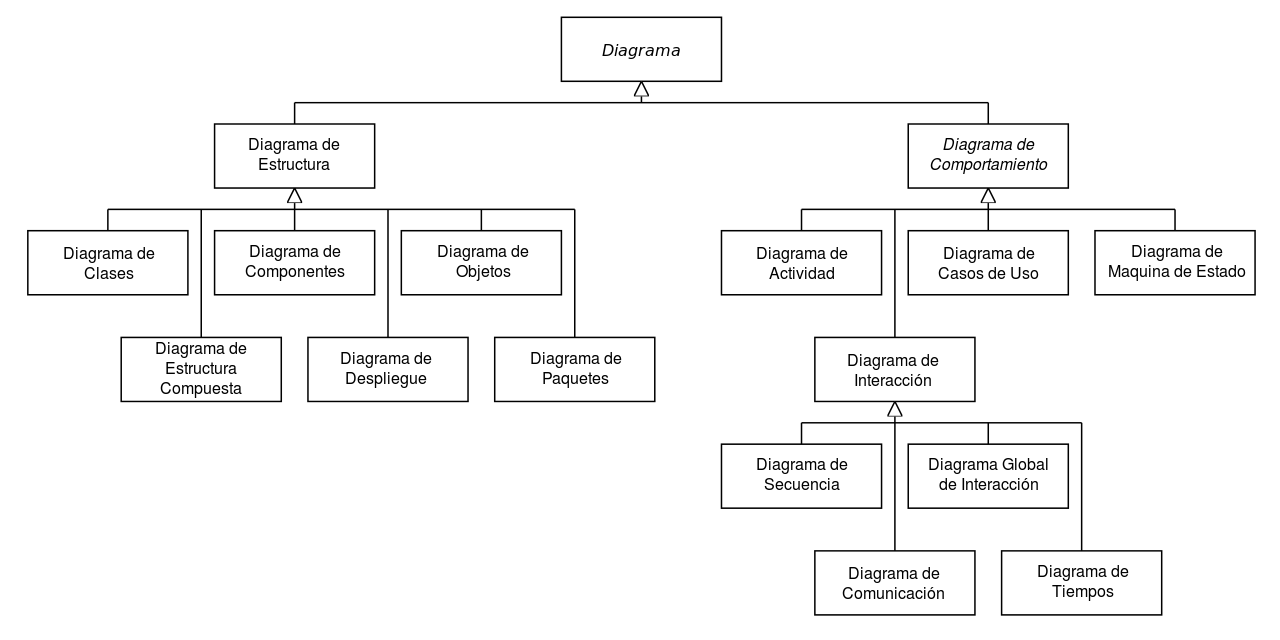
\includegraphics[width=16cm, keepaspectratio]{img/Uml_diagram.png}
	\caption{Jerarquía de diagramas en UML 2.2 (como diagrama de clases).}\label{fig:Uml_diagram}
\end{figure}

\subsection{Diagramas Estructurales}
Los diagramas estructurales muestran la estructura estática de los objetos en un sistema, es decir representan los elementos independientes del tiempo en un sistema. Los diagramas estructurales no muestran los detalles del comportamiento dinámico de un sistema, para ello existen los diagramas de comportamiento, sin embargo, sí que pueden mostrar las relaciones entre los comportamientos definidos en la estructura.  

A continuación, se describe brevemente cada uno de los diagramas pertenecientes a la familia de los diagramas estructurales que se muestran en la Figura~\ref{fig:Uml_diagram}.

\subparagraph{Diagrama de clases}
Este tipo de diagramas proporciona los mecanismos para definir la estructura de un sistema estático. Muestra las clases del sistema, sus atributos, métodos y las relaciones entre los objetos. 
\subparagraph{Diagrama de despliegue}
Esta clase de diagrama muestra la arquitectura de ejecución de un sistema, incluyendo los entornos de ejecución de hardware o software y el middleware que los conecta. Principalmente ayudan a entender y modelar la topología hardware de un sistema y cómo se despliega. 
\subparagraph{Diagrama de componentes} Los diagramas de componentes representan un sistema software dividido en componentes y muestra las dependencias entre los componentes. Son realmente útiles para ver qué componentes pueden compartirse entre sistemas o entre diferentes partes de un sistema.  
\subparagraph{Diagrama de objetos}
Este tipo de diagramas ofrece una vista parcial o completa de los objetos de un sistema. Es un gráfico de instancias que incluye objetos y datos. Estos diagramas están ligados a los diagramas de clases y muestra el estado del sistema en un punto determinado del tiempo. 
\subparagraph{Diagrama de paquetes}
Representa las dependencias entre los paquetes que componen un sistema. Muestra como este está dividido en agrupaciones lógicas y las dependencias entre esas agrupaciones. Estos diagramas muestran la descomposición de la jerarquía lógica de un sistema.  
\subparagraph{Diagrama de estructura compuesta}
Esta clase de diagrama muestra la estructura interna de una clase y las relaciones e interacciones entre las distintas partes de esta. Muestran el rol definido que tiene cada elemento y la estructura compuesta como el conjunto de esos elementos interconectados.
\subsection{Diagramas de Comportamiento}
Los diagramas de comportamiento muestran el comportamiento dinámico de un sistema. Se puede describir como la serie de cambios que pueden existir en un sistema en un tiempo extraordinario.  
\subparagraph{Diagrama de actividad}
También conocidos como diagrama de flujo, contienen la representación gráfica de un algoritmo o proceso. Representan flujos de trabajo paso a paso utilizando símbolos para representar cada uno de estos y flechas que conectan los símbolos para marcar el flujo de ejecución. 
\subparagraph{Diagrama de casos de uso}
Los diagramas de casos de usos describen los diferentes tipos de interacción que tiene alguien o algo con un determinado sistema, especificando el tipo de comunicación y comportamiento de este mediante la interacción con los usuarios y/u otros sistemas.
\subparagraph{Diagrama de interacción}
Este tipo de diagrama describe al detalle un determinado escenario de casos de uso. Ilustran la interacción entre el conjunto de objetos que cooperan en la realización de un proceso. También se pueden utilizar para representar secuencias ordenadas dentro de un sistema. Según las últimas versiones de UML este, diagrama se puede clasificar en cuatro tipos principales de diagramas. 
\begin{itemize}
	\item Diagrama de colaboración. 
	\item Diagrama de secuencia. 
	\item Diagrama de tiempos. 
	\item Diagrama global de interacciones.  
\end{itemize}
Al igual que el resto de diagramas, se hace una introspección más profunda en cada uno de estos diagramas en el Apéndice~\ref{app:diagramas}.
\subparagraph{Diagrama de máquina de estados}
Un diagrama de máquina de estados, conocidos en ocasiones como diagrama de estados, modela el comportamiento de un objeto. Especifican la secuencia de eventos que sufre este determinado objeto durante su tiempo de ejecución. 

\section{Python}
\label{sec:python}
Python~\cite{python} es un lenguaje de programación interpretado, dinámico y multiplataforma con licencia de código abierto\footnote{Python Software Foundation License: \url{https://docs.python.org/3/license.html}}. Su máxima es hacer un lenguaje que sea fácilmente legible y con una empinada curva de aprendizaje. Python fue creado a principios de la década de los 90 por Guido van Rossum en los Países Bajos, como curiosidad, saber que le debe su nombre gracias a la afición que tenía su creador por el grupo de humoristas británicos Monty Python. 

\begin{figure}
	\centering
	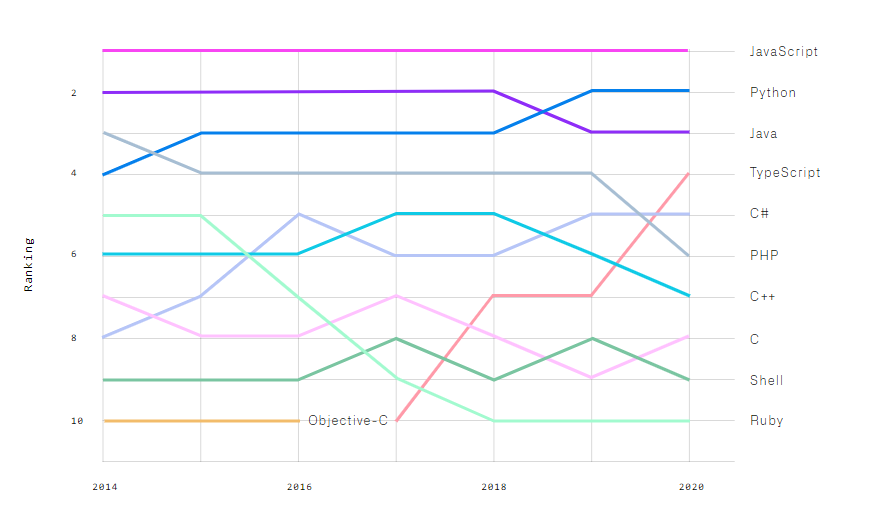
\includegraphics[width=18cm]{img/top_programing_languajes.png}
	\caption{Top uso de lenguajes de programación alojados en GitHub}
	\label{fig:Top_programming}
\end{figure}
%% (source:https://octoverse.github.com/#overview )

Dentro de sus características nos encontramos con que Python es: 
\begin{itemize}
	\item Interpretado: No es necesario que sea procesado por el compilador, se detectan errores en tiempo de ejecución.
	\item Multiparadigma: Soporta tanto programación funcional, como programación orientada a objetos y también programación imperativa.  
	\item Tipado dinámico: Las variables se comprueban en tiempo de ejecución. 
	\item Flexible: No es obligatorio definir ni asignar variables antes de usarlas, es posible omitir parámetros, y su única manera de definir la estructura del código es mediante indentación.
	\item Multiplataforma: Puede ejecutarse tanto en Linux, como Windows como macOS. 
\end{itemize}


La versatilidad y fácil acceso a este lenguaje ha provocado que en los últimos años se haya vuelto muy relevante, haciendo que sea uno de los principales y más importantes lenguajes de programación usados hoy en día. Como se puede ver en la Figura~\ref{fig:Top_programming},
actualmente su última versión estable es Python 3.9, pero este proyecto ha sido desarrollado usando la versión 3.7.3, ya que es una de las más populares y con más usuarios en activo. También cuenta con una versión anterior muy popular, Python 2, que es considerada desactualizada (\emph{deprecated}) desde el 1 de enero de 2020. 

  
\section{Django}
\label{sec:django}
Django~\cite{django} es un framework de desarrollo web gratuito, de código abierto y escrito en Python. Fue lanzado en Julio de 2005 y comparte objetivos generales con Python buscando fundamentalmente poder desarrollar sitios web complejos de manera sencilla y accesible para el mayor número de personan posibles. Django funciona bajo Python, es decir, que para poder trabajar con Django es necesario tener instalado Python. 

Un framework, traduciéndolo al castellano, viene a ser un marco de trabajo, una especie de ecosistema formado por un conjunto de herramientas, librerías y buenas prácticas para crear aplicaciones, en este caso para desarrollar aplicaciones web. 

El framework de Django en concreto nos permite crear sitios web con un cierto grado de complejidad de manera rápida y sencilla. Muchas de las tareas al realizar sitios web suelen ser repetitivas, pesadas y comunes en la mayoría de casos, Django viene a facilitar la realización de estas tareas. 

\subsection{Modelo Vista Controlador (MVC)}
\label{sec:modelo-vista-controlador}
Modelo-vista-controlador es un patrón de arquitectura de software, este patrón consiste en dividir la arquitectura del software en tres grandes módulos: modelo, vista y controlador. Como se ve en la figura~\ref{fig:arquitectura}, en esta figura, las líneas sólidas muestran una relación directa entre los elementos y las rayadas una asociación indirecta.

\begin{itemize}
 \item Modelo: Se encarga de gestionar los datos, normalmente de obtener información de una base de datos. 
 \item Vista: Se encarga de mostrar la información al usuario y las interacciones de este con el sistema. 
 \item Controlador: Gestiona todas las comunicaciones que existen entre la vista y el modelo. 
\end{itemize}

\begin{figure}
	\centering
	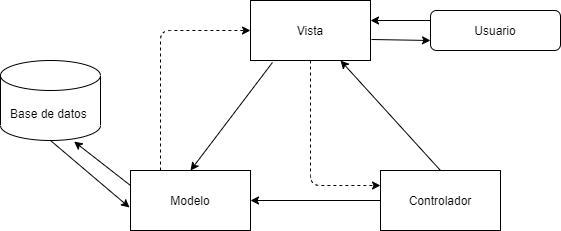
\includegraphics[width=12cm, keepaspectratio]{img/model-vista-controlador.png}
	\caption{Estructura de las relación modelo-vista-controlador.}
	\label{fig:arquitectura}
\end{figure}

Esta división en módulos tiene como ventaja que hace las aplicaciones más funcionales, sostenibles y escalables. Otros muchos grandes frameworks de desarrollo web usan este modelo y, Django, básicamente también, pero llaman a su modelo de manera diferente. La filosofía sigue siendo la del modelo-vista-controlador pero se llama Model Template View, lo que hace es sustituir las vistas por un módulo que llama Template, o plantilla en castellano, el controlador de Django viene a ser el módulo Views y el Model sigue siendo el modelo.

\section{Git}
\label{sec:git}
Git~\cite{git} es un sistema de control de versiones gratuito y de código abierto, diseñado para manejar cualquier tipo de proyecto, tanto en pequeños proyectos como en los muy grandes y complejos, funcionando con gran velocidad y eficiencia. Vino desarrollado por la mano de Linus Torvalds, famoso por iniciar el desarrollo del kernel del sistema operativo Linux. 

Git es fácil de aprender y ocupa poco espacio, con un rendimiento increíblemente rápido. Su objetivo es facilitar el desarrollo y mantenimiento de código fuente tanto de forma individual o como de trabajo en equipo. Te permite crear varias ramas de desarrollo y provee de herramientas para poder unir estas ramas, además de guardar un registro de todos los cambios que sufran los archivos. 

Este software es multiplataforma se puede instalar tanto en Linux, como en Windows y macOS. Se puede utilizar cualquier tipo de lenguaje de programación sobre el archivo del que se desea hacer control de versiones, ya que Git no se fija en el contenido sino en la diferencia de este contenido a lo largo del tiempo y en las diferentes ramas. 

Los repositorios de código que usan Git como control de versiones no necesariamente tienen que estar alojados en un repositorio de Internet, pero lo más habitual y práctico es que sí lo esté. Existen numerosas plataformas que te permiten alojar repositorios de código fuente e interactuar con las herramientas de Git como GitLab o Gogs, que son de código abierto y gratuitas o sitios como CodeComit que pertenece a AWS\footnote{Amazon Web Services} y, por tanto, es de dominio privado. En este proyecto durante su desarrollo se ha utilizado Git para el control de versiones alojando el repositorio en GitHub, que es el otro sitio más de código abierto para alojar proyectos, es gratuita y típicamente se almacenan los repositorios de forma pública.

\section{Bootstrap}
\label{sec:bootstrap}
Bootstrap~\cite{bootstrap} es un framework de código abierto y multiplataforma que contiene bibliotecas y herramientas para el diseño de aplicaciones web. Contiene plantillas de diseño con tipografía, formularios, botones, menús de navegación y otros elementos basados en HTML y CSS, así como extensiones de JavaScript adicionales. Fue desarrollado por Mark Otto y Hacob Thornton como marco de trabajo para fomentar las herramientas internas de Twitter, en 2011 se publicó como código abierto bajo una licencia MIT License.

Bootstrap tiene soporte relativo para HTML5 y CSS3, pero es compatible con la mayoría de los navegadores web. Desde su versión 2.0 soporta diseños web adaptables. Esto significa que el diseño de la web se ajusta dinámicamente en función del display del que disponga el dispositivo donde se esté visualizando, esta tecnología también se conoce como ``responsive'' cuando hablamos de desarrollo web.

Este framework web sólo se ocupa del desarrollo del ``front-end'', es decir de la parte que ve e interactúa el usuario directamente. Integrando este framework con el modelo-vista-controlador de Django, explicado anteriormente en la sección~\ref{sec:modelo-vista-controlador} de este documento podemos enmarcarlo dentro del módulo Template de Django, pudiendo dividir así la parte funcional y práctica del proyecto de la parte del diseño relegándola en Bootstrap. 

\section{Heroku}
\label{sec:heroku}

Heroku~\cite{heroku} es una plataforma que ofrece servicios de computación en la nube que soportan distintos lenguajes de programación. Fue desarrollada en 2007 con el objetivo de soportar la únicamente el lenguaje de programación Ruby, pero poco a poco extendió su soporte para otros lenguajes como Node, Java, PHP y Python entre otros. También soporta servicios de bases de datos tanto MongoDB como Redis o PostgreSQL, tanto como parte de la plataforma como servicio independiente. Además de esto, tiene integración con Git, que, dentro de Heroku, será quien maneje los repositorios de las aplicaciones subidas por los usuarios. 

El modelo de arquitectura de Heroku se basa en Dynos, que son unidades de capacidad de cómputo basadas en contenedores Linux que hay dentro de la plataforma. Cada Dyno está aislado del resto por lo que se pueden desplegar entornos y procesos en cada uno de estos sin que se vean afectado otros. Esto otorga a estas pequeñas máquinas unitarias las siguientes características: 
\begin{itemize}
	\item Elasticidad y crecimiento: La cantidad de Dynos se puede cambiar en cualquier momento. 
	\item Tamaño: Puedes elegir diferentes unidades de memoria y procesamiento en cada máquina. 
	\item Routing: Internamente se conoce la ubicación de los Dynos y, por tanto, redirigen el tráfico eficientemente. 
	\item Seguimiento: Existe un manejador de Dynos, el cual está continuamente monitorizando sus servicios, en caso de que alguno falle este nodo es eliminado y levantado nuevamente. 
	\item Distribución y redundancia. Estas unidades de procesamiento al estar aisladas, implica que, si existen fallos en la infraestructura de una de ellas, las otras no se verán afectadas y en consecuencia tampoco sus servicios. 	
\end{itemize}

Heroku, a diferencia de otras tecnologías vistas en este documento, no es un servicio puramente gratuito, ya que es propiedad de Salesforce, una gran empresa estadounidense de software bajo demanda. No obstante, su unidad de cómputo más básica es de uso gratuito. Con una de estas unidades o Dynos es suficiente para experimentar, poder trabajar en pequeñas aplicaciones y en pruebas de concepto. Todas estas características convierten a este servicio en un entorno perfecto para desplegar una aplicación web pequeña o mediana de manera gratuita, para que esté disponible en cualquier parte del mundo. 
\subsection{Heroku PostgreSQL}
Heroku ofrece la base de datos PostgreSQL, de código abierto, en forma de Heroku Postgres. 

Heroku Postgres~\cite{heroku-postgresql} es una de las soluciones que más usan los desarrolladores en los proyectos de la plataforma. Ofrece todas las ventajas de utilizar PostgreSQL como escalabilidad, acceso a un sistema de administración, seguridad, una alta concurrencia y otras características que se detallan de manera más profunda en la sección \ref{sec:postgeSQL}

Los planes de precio que Heroku ofrece a sus usuarios para este servicio pasan por una gran variedad de precios, pero cuenta con un plan gratuito para desarrolladores que permite probarlo sin ningún riesgo con un tamaño y características más que suficientes para pequeños proyectos o pruebas de concepto sencillas. 

\section{SQLite 3}
\label{sec:SQLite}

SQLite~\cite{sqlite} es un sistema de gestión de bases de datos relacional de código abierto.  A diferencia de los sistemas de gestión de bases datos cliente-servidor, la biblioteca SQLite es una parte integral del programa que enlaza, y no un proceso independiente del mismo. Esto hace que la latencia sea más reducida y las comunicaciones entre procesos y funciones son más eficientes. 

SQLite nació en el año 2000, fue creado por D. Richard Hipp y su objetivo era diseñar un sistema de gestión de bases de datos relacional que permitiera ejecutar programas sin la necesidad de instalar un sistema de gestión de bases de datos. 

Sus primeras versiones se caracterizaban por contener la base de datos en un espacio en disco relativamente pequeño y está contenida en un solo archivo. En su versión 3, SQLite admite bases de datos de hasta 2 Terabytes de tamaño. 

Este sistema de gestión de bases de datos soporta funciones SQL definidas por los usuarios, y tiene otras ventajas como una amplia compatibilidad con diferentes plataformas como Windows, Linux, Android, MacOS e iOS. También es compatible con casi todos los lenguajes de programación y proporciona APIs útiles para ellos. Por defecto, es la base de datos que viene configurada para proyectos de Django, por su ligereza, independencia de paquetes externos y la eficiencia de sus procesos es ideal para pruebas de concepto en proyectos pequeños, pero es difícil de escalar y al no presentar el estándar cliente-servidor tiene limitaciones en cuanto al formato y la sintaxis, y no presenta muchas funciones de seguridad.

Este tipo de base de datos es la seleccionada por defecto al comenzar proyectos en Django. Es por eso que se optó en un primer momento desarrollar el proyecto con este tipo de base de datos. Más adelante, en un punto avanzado del desarrollo, fue necesario implementar la compatibilidad con una base de datos de tipo PostgreSQL para el despliegue del proyecto en Heroku. Actualmente, este software es compatible con ambos sistemas de gestión de bases de datos.

\section{PostgreSQL}
\label{sec:postgeSQL}
PostgreSQL~\cite{postgresql}, también llamado Postgres, es un sistema de gestión de bases de datos relacional orientado a objetos y de código abierto. Este proyecto de código abierto no es gestionado por una persona o empresa, sino que lo mantienen una comunidad de desarrolladores que trabajan de forma altruista y libre, el PGDG.\footnote{PostgreSQL Global Development Group}

Entre las características principales de este sistema de gestión de bases de datos se encuentran: 
\begin{itemize}
	\item Alta concurrencia: Permiten que varios usuarios o procesos accedan a la misma tabla sin necesidad bloqueos. 
	\item Amplia variedad de tipos nativos: PostgreSQL provee nativamente soporte para diferentes tipos de datos como texto ilimitado, direcciones IP o MAC o CIDR, arrays, números de precisión arbitraria e incluso figuras geométricas (con variedad de funciones asociadas). Adicionalmente, permite que los usuarios puedan crear sus propios tipos de datos, que se pueden indexar perfectamente a una tabla. 
	\item Otras características deseables en un gestor de bases de datos, como claves foráneas (\emph{foregin keys}), disparadores, herencia de tablas, integridad transaccional, seguridad y escalabilidad.  
\end{itemize}
Las ventajas que ofrece este gestor de base de datos son básicamente seguridad e integridad en términos generales en la BD\footnote{Base de Datos}, un buen sistema de transacciones y respaldos y una conexión al sistema de gestión de base datos. Desafortunadamente, no cuenta con gestor de errores, por tanto, es difícil conocer el estado de los errores o corregirlos. 

Como ya vimos en el \ref{sec:heroku}, PostgreSQL cuenta con un paquete propio integrado en Heroku que permite utilizar este sistema de gestión de bases de datos junto con el almacenamiento de los mismos en servicios virtualizados de manera gratuita en algunos de sus planes.  

\section{Visual Studio Code}
Visual Studio Code~\cite{vscode} es un editor de código fuente, lanzado en 2015 y desarrollado por Microsoft. Es un editor multiplataforma compatible con Windows, Linux, MacOS y ahora cuenta también con una versión web. 

Soporta prácticamente cualquier lenguaje de programación conocido, resaltando la sintaxis de este de manera personalizada, ofrece sugerencias de sentencias y variables, finalización inteligente de código, integración con la shell y un gestor de archivos interno. Incluye soporte para depuración y control de versiones integrado con Git. Además, gracias a la gran comunidad de desarrolladores, existen infinidad de \emph{plugins} muy fácilmente instalables que añaden funcionalidades realmente útiles a la hora de programar, depurar, integrar o desplegar código. 
Es un software gratuito y de código abierto pero la descarga oficial está bajo software privativo de Microsoft. 

Visual Studio Code recopila datos de uso y los envía a Microsoft, aunque esto se puede desactivar, y por la naturaleza open-source de la aplicación se puede ver exactamente qué clase de datos se recopilan y envían. Los datos pueden ser compartidos entre Microsoft, sus filiales y las autoridades según lo firmado conformemente en la declaración de privacidad. 

\section{WSL 2}
\label{sec:WSL}
Windows Subsystem for Linux (WSL)~\cite{wsl2} es una capa de compatibilidad entre sistemas desarrollada por Microsoft con el objetivo de poder correr ejecutables de Linux nativamente en Windows 10 y Windows Server. En 2019 se lanza la versión 2 de WSL incluyendo cambios importantes, como el uso real del kernel de Linux. 

WSL ofrece una interfaz que simula el kernel de Linux sobre Windows sin necesidad de instalar un SO\footnote{Sistema Operativo} en particiones de disco y sin necesidad de crear una máquina virtual que tenga que emular hardware. Establece un espacio de usuario GNU\footnote{GNU es un sistema operativo de tipo Unix, así como una gran colección de programas informáticos que componen al sistema, desarrollado por y para el Proyecto GNU y auspiciado por la Free Software Foundation.} donde instalar un sistema base como Ubuntu, Debian o Kali Linux. Dicho entorno no contará con interfaz gráfica(a no ser que tenga ayuda de aplicaciones gráficas como un servidor X11) sino que se accederá a ella mediante una Shell de tipo Bash\footnote{Bash (Bourne-again shell) es una popular interfaz de usuario de línea de comandos, específicamente un Shell de Unix; así como un lenguaje de scripting}. 

Para acceder al hardware y al sistema de archivos, se hace uso directo del sistema de archivos en Windows y partes del hardware como el hardware de red e incluso su infraestructura como los puertos. Este uso compartido del sistema hace que haya gran interoperabilidad entre ambos. Esto permite incluso desarrollar software sobre Linux, en un sistema Windows con sus aplicaciones propias como Visual Studio, hacer que ejecute el código en un entorno Linux con sus respectivos paquetes de software y acceder al programa o aplicación desarrollado a través de un puerto de red en un navegador de Windows con relativa facilidad. 

\section{Diagrams.net}
Diagrams.net~\cite{diagrams.net}, anteriormente conocido como draw.io, es un software de código abierto de dibujo gráfico, pensado especialmente para la creación y dibujado de diagramas.

Está desarrollado en HTML5 y JavaScript, es multiplataforma y está disponible en aplicación web\footnote{https://app.diagrams.net/}. Aparte de ser muy intuitiva y fácil de manejar, no requiere inicio de sesión o registro. Permite exportar los diagramas o dibujos a gran cantidad de formatos como .PNG, .PDF, .SVG y .JPEG. Se puede integrar con servicios de almacenamiento \emph{onCloud} como Google Dive, Dropbox o OneDrive (para estas funcionalidades sí es necesario registrarse) y cuenta con un complemento para integrar la aplicación web en Visual Studio Code, lo cual simplifica el poder hacer diagramas UML paralelamente al desarrollo de un software.


%%%%%%%%%%%%%%%%%%%%%%%%%%%%%%%%%%%%%%%%%%%%%%%%%%%%%%%%%%%%%%%%%%%%%%%%%%%%%%%%
%%%%%%%%%%%%%%%%%%%%%%%%%%%%%%%%%%%%%%%%%%%%%%%%%%%%%%%%%%%%%%%%%%%%%%%%%%%%%%%%
% DISEÑO E IMPLEMENTACIÓN %
%%%%%%%%%%%%%%%%%%%%%%%%%%%%%%%%%%%%%%%%%%%%%%%%%%%%%%%%%%%%%%%%%%%%%%%%%%%%%%%%

\chapter{Diseño e implementación}
\label{chap:diseño}


\section{Arquitectura general} 
\label{sec:arquitectura}

La aplicación web \texttt{Gymkhana App} se ha desarrollado en Django con su estructura típica basada en el modelo-vista-controlador, que se explica más detalladamente en la sección~\ref{sec:modelo-vista-controlador}. Dentro de este modelo, la vista será la capa que se presente y con la que interactúa el usuario, compuesta por los diferentes tipos de plantillas o Templates como los conoce Django. El modelo es quien se encarga de gestionar los datos, es quien tiene comunicación directa con la base datos y maneja toda la información que entra y sale de esta. El controlador es quien maneja las comunicaciones entre los dos anteriores módulos y el único que tiene conexión directa con el resto de los módulos, se encarga de recibir las peticiones del módulo de vistas, gestionar internamente estas peticiones y decidir qué hacer en base a la información recogida consultando en cualquier caso los datos que considere necesarios del modelo. 


\section{Módulo Vistas-Controlador}
Este módulo es el encargado de recibir y gestionar las peticiones recibidas desde el módulo Templates, gestionarlas, consultar con el módulo Models y preparar las respuestas para el usuario. Django dispone de herramientas muy útiles para la gestión y respuesta de peticiones web, de tal manera que definir las funciones del servidor cada vez que un usuario accede a una URL y generar las respuestas es limpio, sencillo, escalable. 
Las URL y como se gestionan las respuestas se define a continuación: 

\begin{itemize}
	\item \textbf {/ (Home)}: Como muchas otras aplicaciones que existen, cuando se introduce la URL con el nombre completo del dominio sin añadir ningún directorio tras este, se nuestra la página principal o home, donde, simplemente, se pueden ver dos botones grandes. Uno de ellos permite iniciar sesión y registrarte, y el otro, iniciar Gymkhana App.
	\item \textbf {/start}: Cuando accedes a la aplicación desde el home te lleva automáticamente a esta dirección, donde primero este módulo comprueba si existen juegos disponibles en la base de datos, y si es así, los muestra. El usuario puede elegir uno de estos juegos y enviar una petición GET con el identificador del juego elegido. 
	\item \textbf {/challenge}: Cuando se accede a este directorio, se recoge la petición GET del usuario con el juego seleccionado, y si vienes de un reto anterior o acaba de empezar el juego. Así podemos elegir cuál de los diferentes retos que componen un juego mostrar, siempre comprobando que todos los datos existan en la base de datos para evitar posibles errores. Una vez elegido el reto a mostrar se le muestra el reto donde el usuario debe introducir la respuesta de este para poder avanzar. 
	\item \textbf {/response}: Una vez el usuario ha rellenado la repuesta al reto se envía una petición tipo GET con la información contenida del reto al que pertenece, el juego, si ha habido un reto del mismo juego anterior y la respuesta al reto. En caso de ser correcta el servidor redirigirá al usuario al nuevo reto, si se está jugando a un juego con varios retos, o a una pantalla en la que indica que ha finalizado correctamente el juego y desde ahí el usuario podrá regresar al menú principal para poder elegir otros juegos, o repetir el mismo. También en cada response se analizará si el usuario que está jugando está registrado y le añadirá a ese usuario la puntuación de dicho reto, pero solo en caso de que no lo haya completado anteriormente. Por otro lado, si la respuesta no es correcta, enviará al usuario a una pantalla donde se indica que la respuesta es incorrecta y te dejará volver a intentar el reto o salir al menú de juegos.
	\item \textbf {/accounts}: Esta dirección funciona de una manera un poco diferente. Para el inicio de sesión, modificación de contraseñas y cierre de la misma en la aplicación se ha decidido utilizar un módulo ya implementado de Django que gestione correctamente estas peticiones. Este módulo se le conoce como ``Django’s authentication system'' y está dentro de la configuración por defecto de Django. Una vez accedemos a esta dirección el usuario deberá ingresar su nombre de usuario y contraseña para poder continuar. En caso de ser correcto redirigirá al usuario a su perfil. Cuando el usuario decida cerrar la sesión se le redirigirá al home de la aplicación. 
	\item \textbf {/profile}: Si te registras en la aplicación exitosamente podrás acceder a tu perfil de usuario a través de una petición GET en esta dirección. Básicamente aquí se muestra la información del usuario, como el nombre o el acumulado de sus puntos. También se podrá acceder a /start para comenzar a jugar. Desde este punto el usuario que ha iniciado sesión puede acceder a los módulos para crear retos y juegos 
	\item \textbf {/create challenge}: En esta dirección primero comprueba que el usuario esté registrado y si es así se le muestra un formulario con los campos necesarios que componen un reto. Para poder continuar desde este punto habrá que haber rellenado correctamente todos los datos del formulario y pulsar el botón de subir reto. 
	\item \textbf {/upload challenge}: La activación de botón mencionado en el apartado anterior enviara los datos del formulario mediante una petición POST. En este punto se revisa que los campos requeridos hayan sido rellenados correctamente y en caso afirmativo se guarda este reto en base de datos.  
	\item \textbf {/create game}: Al igual que para crear un reto, se accede a este módulo desde la página del usuario, una vez se haya registrado. En este caso, una vez se haya accedido se presenta un formulario para poder crear un juego. Como los juegos son simples colecciones de retos, aquí se le muestra al usuario un listado con los retos subidos para que seleccione uno o varios retos. La única forma de avanzar desde este punto será pulsando el botón de subir juego con el formulario correctamente cumplimentado. 
	\item \textbf {/upload challenge} Para terminar la subida de un juego se envían los campos del formulario contenidos en una petición POST que será la se espera recibir aquí. En caso de que todos los campos requeridos existan y sean correctos subirá el juego a la base de datos de la aplicación Gymkhana App.
	
\end{itemize}

Django cuenta con muchas funciones y respuestas que vienen ya integradas, como por ejemplo poder responder a peticiones que provocan errores genéricos como tipo HTTP 404 (Not Found), entre otros. De esta manera todas las peticiones que se hacen al servidor en caso de no encontrar la información requerida en la base de datos la aplicación captura este error y devuelve un ERROR 404 genérico de Django, que aparte hace terminar el resto de procesos en curso, haciendo a la aplicación mucho más robusta ante errores. 


\section{Módulo Templates-Vistas}
El módulo de Templates es el que forma la interfaz de usuario de la aplicación. Cada vista de la aplicación, o página que el usuario acaba visualizando. Está compuesta por un template o plantilla HTML sobre la que se aplica un estilo con CSS. Trabajar con plantillas en Django hace que la aplicación sea escalable y el código quede ordenado. En muchos casos la plantilla es reutilizable si se parametrizan adecuadamente, a su vez, la capa de estilo está muy bien aislada gracias a Bootstrap, de manera que se puede separar muy bien la parte programática del desarrollo de la parte encargada del diseño y el estilo evitando así tener que aplicar estilo a cada una de las páginas implicadas en el desarrollo. 

La aplicación de \texttt{Gymkhana App} se compone de las siguientes views: home, start, challenge, succes y wrong, login, profile, create challenge y create game
\subparagraph{Home}
Es la página principal que el usuario ve cuando accede a la web. Se limita a una presentación sencilla y limpia del proyecto, con un botón bien visible al usuario que será el que le permita avanzar y adentrarse en Gymkhana App. 
\subparagraph{Start}
Esta página actúa de forma de menú y muestra los juegos que hay disponibles en la aplicación, los lista ordenadamente de manera descendientes, y cada juego tiene un botón con el que él usuario puede interactuar, pulsando el mismo se accede a dicho juego.  
\subparagraph{Challenge} 
En esta página muestra un único reto, que se compone de un nombre o título, una pregunta y una imagen con un diagrama UML que debe estar relacionado con el reto. Esta vista tiene también un campo que el usuario debe rellenar con la respuesta planteada al reto y un botón para enviar la petición que más tarde procesará el módulo Vistas-Controlador.
\subparagraph{Success}
Una vez enviada la respuesta a un reto, si eta es correcta te redirigirá a esta página donde puedes ver un texto dando la enhorabuena al usuario. Dependiendo del juego te mostrará un botón para volver al menú de juegos o al siguiente reto si el juego estaba compuesto por varios. 
\subparagraph{Wrong}
En contraposición a la anterior plantilla, esta mostrará al usuario un comentario haciéndole saber que la respuesta no es correcta, pero también animándolo a que lo vuelva a intentar. Esta plantilla solo mostrará dos botones, uno para volver a intentar el reto que ha fallado y otro para volver al menú de juegos en caso de que el usuario desista y de por perdido el reto. 

\subparagraph{Login}
Tiene la estructura de cualquier página de inicio de sesión tradicional, donde el usuario deberá introducir su nombre y contraseña para acceder. Como diferencial al resto de sitios web, \texttt{Gymkhana App} no ofrece en esta página la opción de crear un usuario, ya que un usuario registrado tiene la capacidad de hacer inyecciones en la base de datos y subir contenidos como imágenes. Por tanto y por motivos de seguridad, la potestad de creación de usuarios queda relegada solo al administrador de este proyecto que, en todo caso, proporcionara las credenciales de registro a quien considere necesario.   

\subparagraph{Profile} Una vez el usuario esté registrado tendrá acceso a esta página, donde podrá ver información del usuario, como su nombre en la aplicación y los puntos que ha obtenido. Además, desde este punto tendrá acceso a las dos siguientes views: create challenge y create game

\subparagraph{Create Challenge} En esta página se podrá ver un formulario con los campos que debe rellenar un usuario para poder subir el reto. Los campos son los siguientes:
\begin{itemize}
	\item \textbf {nombre}: Nombre o título deseado para el reto.
	\item \textbf {pregunta}: Será la cuestión a la que los jugadores deban responder para poder completar el desafío.
	\item \textbf {solución}: La respuesta o solución correcta que se espera por parte del jugador para poder completar el reto.
	\item \textbf {tipo de diagrama}: En este campo se despliega una lista con todos los tipos de diagramas UML para que el usuario que está subiendo el juego seleccione el tipo de diagrama al que pertenece el usado en el reto.
	\item \textbf {imagen}: Un campo que permite al usuario abrir el explorador de archivos de su sistema operativo para poder subir una imagen, en concreto se debe subir la imagen del diagrama UML asociado al reto. 
	\item \textbf {puntos}: Valor que se le quiere dar en puntos al reto.
\end{itemize}	

\subparagraph{Create Game} Al igual que la anterior esta página mostrará un formulario que se deber rellenar para poder crear juegos. 
\begin{itemize}
	\item \textbf {título}: Nombre o título deseado para el juego.
	\item \textbf {retos}: Se muestra una lista con todos los retos subidos a la plataforma, tanto los creados por ese usuario como los creados por otros. El usuario que cree un juego puede elegir uno o tantos como considere para formar un juego. 
\end{itemize}	


Todas estas páginas han sido construidas sobre una base genérica común que usan todas las plantillas. Esta base común permite contener la información de todas las vieews mencionadas anteriormente, además de la cabecera o ``header'' y el pie de página o ``footer''. En la cabecera hay dos enlaces ocultos que redirigirán al usuario bien a la página principal de la aplicación Gymkhana App, o a la web oficial de la organización UML. En el pie de página se muestra información relativa a la ETSIT como localización y enlaces ocultos para poder visitar la cuenta de Twitter, y la web oficial de la ETSIT. También aparece la licencia de uso de la plantilla de Bootstrap elegida

\subsection{Internacionalización}
Django también ofrece de manera relativamente sencilla la posibilidad de añadir internacionalización a las plantillas. Este proceso consiste en traducir todo el texto que aparece en las plantillas. 

En este proyecto, el idioma original que se eligió para desarrollar las plantillas fue el inglés, pero con el proceso de internacionalización también está disponible en castellano. La idea básica de la internacionalización o i18n es marcar aquellas cadenas de texto que deben ser traducidas. Estas cadenas se guardan en un diccionario, donde se añade la traducción al idioma o idiomas deseados, de esta manera cuando un usuario seleccione un idioma, mostrará estas cadenas de texto marcadas en el lenguaje que le corresponda al usuario. 

En el diccionario, aparte de todas las cadenas de texto que se muestran en las diferentes plantillas, también están guardadas las respuestas a los retos. Esta es la única manera de poder procesar las respuestas de los usuarios en diferentes idiomas y comprobar que coinciden con la respuesta de un reto concreto. 


\section{Módulo Models-Modelo}
Este módulo es el que gestiona la información de la aplicación Gymkhana App, toda la información de la aplicación está contenida en una base de datos. El gestor de base de datos utilizado es, en este caso, SQLite versión 3. Este sistema de base de datos es un sistema de base de datos relacional y es por defecto el que utiliza Django, no obstante, se permite cambiar a otros modelos fácilmente. Se ha decidido utilizar este gestor precisamente por la sencillez y compatibilidad con Django. Con SQLite la base de datos completa se encuentra en un solo archivo totalmente autocontenido, sin dependencias externas, además, admite concurrencia, es decir, que permite que múltiples procesos tengan el archivo de base de datos abierto y puedan leer a la vez. En la figura~\ref{fig:diagarma_ER} se puede ver el diagrama entidad-relación que define la base de datos de la aplicación, el proyecto de Django tiene más tablas aparte de las que se muestran, pero el resto son propias de la arquitectura de Django así que no nos centraremos en ellas. Las tablas que componen la base de datos de la aplicación se describen a continuación:


\begin{itemize}
	\item \textbf {Users}: En esta tabla se almacenan los usuarios registrados en Gymkhana App. Dispone de los siguientes campos: 
	\begin{itemize}
		\item \textbf {name}: Indica el nombre del usuario. 
		\item \textbf {email}: La dirección de correo electrónico con la que se registra el usuario. 
		\item \textbf {admin}: Un campo que indica si este usuario tiene privilegios de administrador o no. 
		\item \textbf {points}: Campo numérico entero que contiene la puntuación del usuario. 
		\item \textbf {challenges passed}: Un relación Many To Many con la tabla Challenges, que registra que Challenges ha superado ya el usuario. 
		\item \textbf {created at}: Campo en formato fecha del momento en el que se crea el usuario. 
		\item \textbf {updated at}: Campo en formato fecha que indica el momento que se actualiza la información del usuario. 
	\end{itemize}

	\item \textbf {Diagrams}: Esta tabla contiene los tipos de diagramas que pueden aparecer en los retos, estos tipos de diagramas se limitan a los mencionados en el apartado 3.1 de este documento.  
	\begin{itemize}
		\item \textbf {name}: Indica el nombre general del tipo de diagrama UML. 
		\item \textbf {description}: La descripción del tipo de diagrama asociado que se puede extender hasta diez mil caracteres. 
	\end{itemize}
	
	\item \textbf {Challenges}: Tabla que almacena los retos de los que se componen los juegos que maneja la aplicación. 
	\begin{itemize}
		\item \textbf {name}: Nombre que se le da a cada reto.
		\item \textbf {question}: Pregunta clave sobre el reto específico. 
		\item \textbf {awnser}: Respuesta a la pregunta clave. 
		\item \textbf {image}: 	Campo tipo imagen que contiene el Diagrama UML al que está asociado el reto. 
		\item \textbf {diagram type}: Identificador único que referencia el tipo de diagrama de la tabla Diagrams al que está asociado el reto. 
		\item \textbf {creator}: Usuario que ha creado este reto. 
		\item \textbf {created at}: Campo de tipo date que registra el momento en el que se creó el reto. 
		\item \textbf {points}: Campo tipo numérico entero que contiene la puntuación del reto. 		
	\end{itemize}
	
	\item \textbf {Games}: Tabla que almacena los distintos juegos, estos juegos son principalmente una colección de uno o varios retos. 
	\begin{itemize}
		\item \textbf {title}: Nombre o título del juego. 
		\item \textbf {challenges}: Uno o varios retos de los contenidos en la tabla Challenges. 
		\item \textbf {creator}: Usuario que ha creado el juego. 
	\end{itemize}
	
\end{itemize}

\begin{figure}
	\centering
	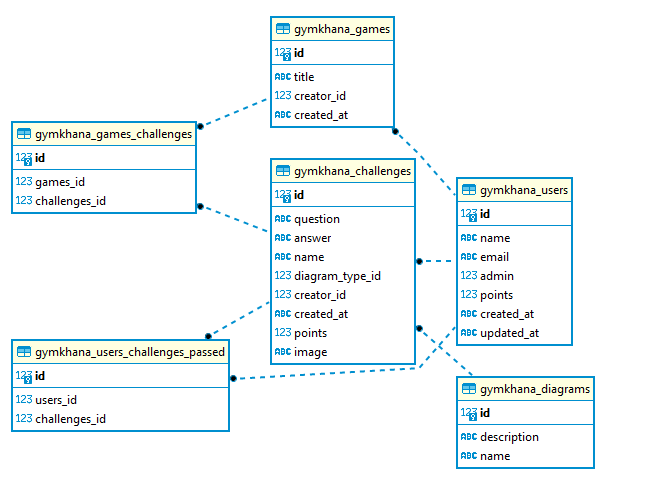
\includegraphics[width=16cm, keepaspectratio]{img/gymkhana_ER.png}
	\caption{Diagrama entidad-relación de la aplicación Ghymkhana App.}\label{fig:diagarma_ER}
\end{figure}

\section{Despliegue del software}
\label{sec:despliegue}
Con el objetivo de poder acceder a \texttt{Gymkhana App} desde cualquier lugar con acceso a la red de Internet, este proyecto se ha desplegado en un servidor de acceso público. Este despliegue se ha realizado en los servidores de Heroku, se puede encontrar más información acerca de este servicio en la sección~\ref{sec:heroku}. 

Heroku ofrece varias maneras de gestionar el despliegue de código en sus servidores; con un proyecto Git, a través de Docker\footnote{Herramienta de automatización de despliegue de software en contenedores que se ha hecho muy popular en estos últimos años entre los desarrolladores.} y con otros servicios de integración populares entre desarrolladores. En este proyecto se ha desplegado en Heroku a través de Git.

Para este proceso de despliegue es por tanto necesario tener instalado en la máquina desde la que se quiere desplegar el proyecto los paquetes de Git y Heroku CLI. Además de hacer ciertas variaciones en el proyecto y añadir archivos necesarios para la autoconfiguración en las máquinas remotas de Heroku. Estas modificaciones se explican a continuación: 

Heroku necesita saber el lenguaje o lenguajes de programación en el que está basado el proyecto, para esto, es necesario crear en la carpeta raíz del proyecto un archivo llamado \emph{runtime.txt}, en el caso particular de este proyecto este archivo está compuesto de una sola línea. 
\begin{verbatim}
	python-3.7.13
\end{verbatim}

También será necesario añadir en el archivo \emph{requirements.txt} todas las dependencias del proyecto para que Heroku pueda instalarlas. Es importante durante el proceso de desarrollo haber tenido un entorno aislado y tener todas las dependencias del proyecto correctamente instaladas. 
\begin{verbatim}
	$ pip freeze > requirements.txt
\end{verbatim}

Para que las máquinas de Heroku tengan la información necesaria para ejecutar las piezas de la aplicación es necesario un archivo \emph{Procfile}. En el caso de este proyecto se compone como se indica a continuación:
\begin{verbatim}
	web: gunicorn ProjectUML.wsgi 
\end{verbatim}

Para que en el servidor tenga archivos estáticos es necesario editar el fichero de \emph{settings.py} y añadir el siguiente \emph{middleware}, su función es básicamente para mejorar la eficiencia de la aplicación, comprimiendo y almacenando en caché información de los ficheros estáticos del proyecto.
\begin{verbatim}
	STATICFILES_STORAGE = 
	'whitenoise.storage.CompressedManifestStaticFilesStorage'
\end{verbatim}

Una vez hecho todo esto, suponiendo que el repositorio del proyecto ya tenga una rama Git iniciada para el control de versiones y que el usuario se haya registrado dándose de alta en Heroku, se enlazará el directorio Git con el proyecto existente en Heroku de manera local.
\begin{verbatim}
	$ heroku create -a project-uml 
	  # si el proyecto ya existe se debe usar este otro comando: 
	$ heroku git:remote -a project-uml 
	$ git add -A
	$ git commit -m "cambios para despliegue en Heroku"
	$ git push heroku main
\end{verbatim}

En este momento, el proyecto ya estaría desplegado y listo para usarse, sin embargo, no tendría nada de información contenida en la base de datos, aunque sí tendrá su estructura formada. Es necesario migrar la base de datos local usada en desarrollo hacía la base de datos PostgreSQL.
\begin{verbatim}
	$ python3 manage.py dumpdata --exclude contenttypes > data.json
	$ git add data.json
	$ git commit -m "se añade archivo para migración de base de datos."
	$ git push heroku main
	$ heroku run python3 manage.py loaddata data.json
\end{verbatim}




%%%%%%%%%%%%%%%%%%%%%%%%%%%%%%%%%%%%%%%%%%%%%%%%%%%%%%%%%%%%%%%%%%%%%%%%%%%%%%%%
%%%%%%%%%%%%%%%%%%%%%%%%%%%%%%%%%%%%%%%%%%%%%%%%%%%%%%%%%%%%%%%%%%%%%%%%%%%%%%%%
% RESULTADOS %
%%%%%%%%%%%%%%%%%%%%%%%%%%%%%%%%%%%%%%%%%%%%%%%%%%%%%%%%%%%%%%%%%%%%%%%%%%%%%%%%

\cleardoublepage
\chapter{Resultados}


\label{chap:resultados}

\section{Acceso al proyecto}

Se puede acceder a \texttt{Gymkhana App} a través del siguiente enlace: 
\begin{itemize}
	\item \url{https://project-uml.herokuapp.com/}
\end{itemize}
Y el código fuente utilizado se encuentra en un repositorio público de GitHub: 
\begin{itemize}
	\item \url{https://github.com/jorgedepablo/ProjectUML}
\end{itemize}

\section{Página principal}
La página principal, también comúnmente conocida como \emph{home}, tiene la única función de presentar la aplicación de manera clara y limpia, con no demasiada información para no bombardear ni agobiar a los potenciales usuarios que puedan visitar la página. En este punto también se exponen dos botones principales que llevan a las dos principales funcionalidades de la aplicación: empezar a jugar y poder registrarse para acceder a las funcionalidades que permiten crear nuevos retos y juegos. 

\begin{figure}
	\centering
	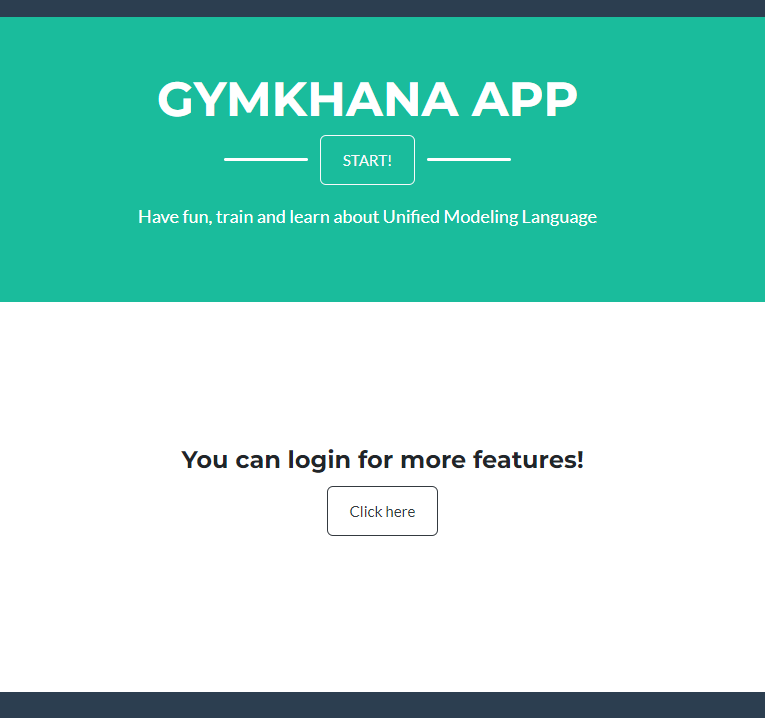
\includegraphics[width=16cm, keepaspectratio]{img/home_html.png}
	\caption{Página principal de la aplicación.}\label{fig:home}
\end{figure}

\section{Menú de juegos}
El menú de juego es la página a la que accedes inmediatamente después de pulsar el botón \emph{START!} de la página principal. Aquí se presentan en manera de lista descendiente todos los juegos subidos a la aplicación. Pulsando sobre la imagen de cada uno de los juegos la aplicación debería llevar al usuario al primer reto de cada una de las pruebas. 

\begin{figure}
	\centering
	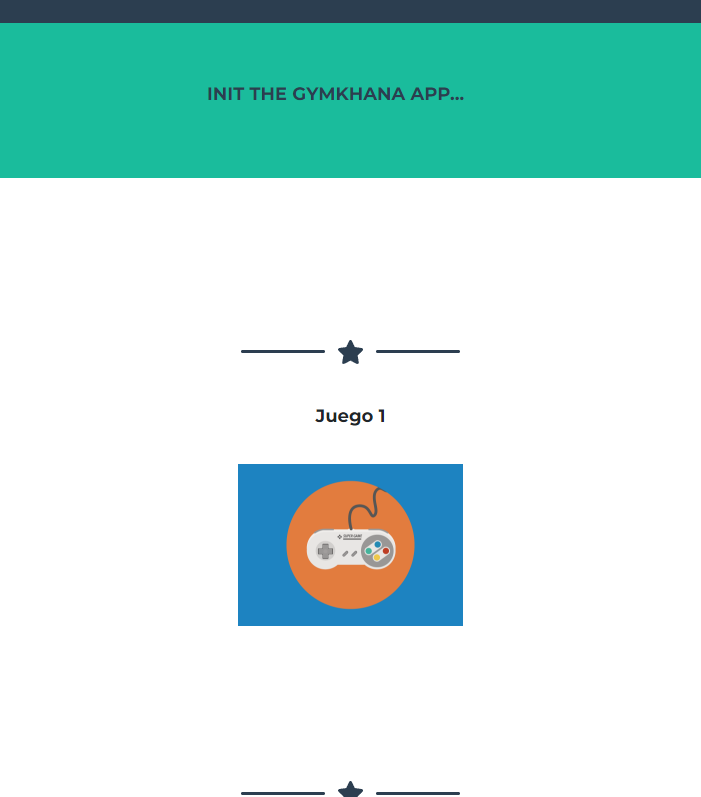
\includegraphics[width=16cm, keepaspectratio]{img/start_html.png}
	\caption{Menú de juegos de la aplicación.}\label{fig:start}
\end{figure}

\section{Página de los retos}
Una vez pulsado sobre uno de los juegos redirigirá al usuario a la página con el primer reto del juego seleccionado. Todos los retos siguen el mismo esquema: 
\begin{enumerate}
	\item En la cabecera del reto se ve el nombre del tipo de diagrama UML con el que está relacionado el reto.
	\item Para abrir el reto tenemos un pequeño resumen explicando el tipo de diagrama que es y para qué sirve. 
	\item Luego se plantea la pregunta o tarea a la que debe responder el usuario para poder completar el reto. 
	\item Debajo está la imagen con el diagrama UML sobre el cual el usuario debe extrae la información para poder contestar el reto.
	\item Por último, un cuadro de texto y un botón de enviar la respuesta. 
\end{enumerate}
Después de enviar la respuesta el usuario es redirigido a otra página donde se le dice al usuario si la respuesta es correcta o no. En caso de que sea correcta el usuario podrá continuar con el siguiente reto, si es que el juego está formado por más, y en caso de que sea incorrecta, se le da la opción de volver al menú de juegos o volver a intentar el reto fallado. 
\begin{figure}
	\centering
	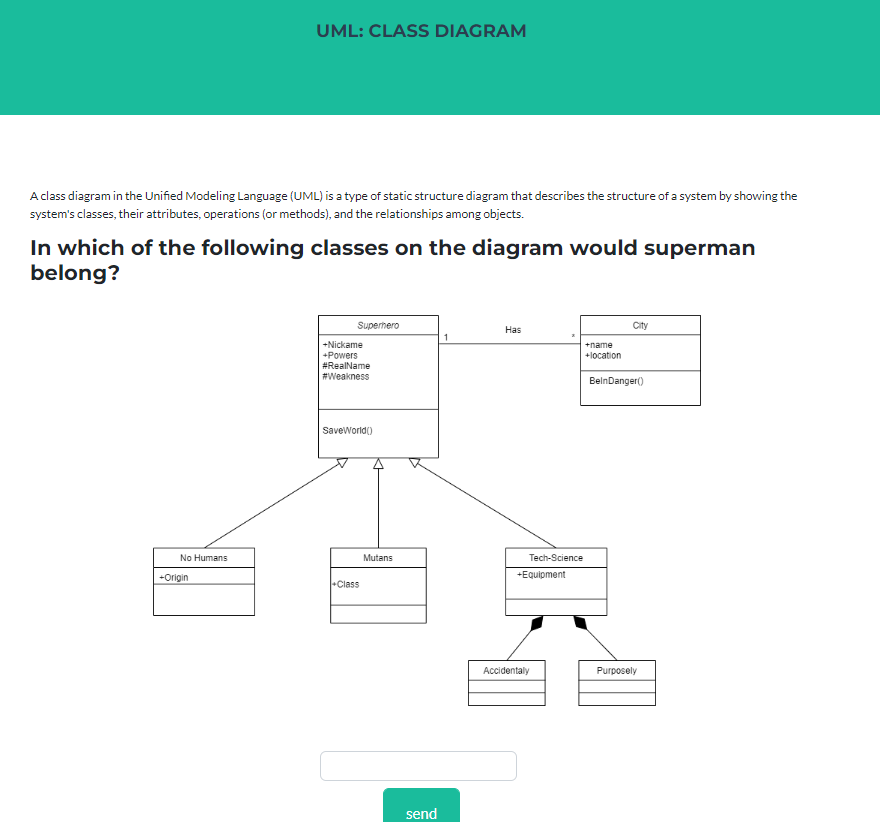
\includegraphics[width=16cm, keepaspectratio]{img/challenge_html.png}
	\caption{Ejemplo de un reto.}\label{fig:challenge}
\end{figure}

\section{Inicio de sesión}
La sección de inicio de sesión se reduce a un simple \emph{login}. Por motivos de seguridad no se ha implementado las funcionalidades de registro o dar de alta a un nuevo usuario. El uso es simple; el usuario debe introducir las credenciales dadas por el administrador de la aplicación y pulsar el botón de iniciar sesión. 
\begin{figure}
	\centering
	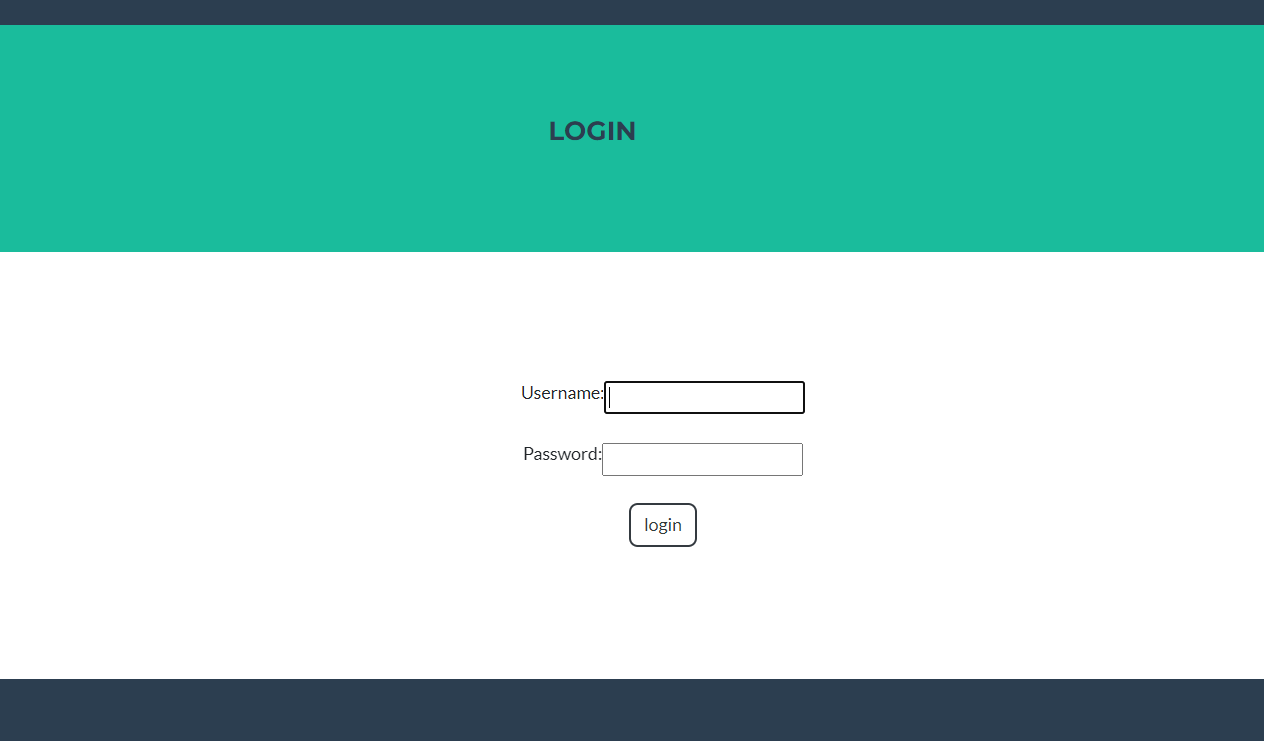
\includegraphics[width=16cm, keepaspectratio]{img/login_html.png}
	\caption{Página de inicio de sesión.}\label{fig:login}
\end{figure}

\section{Perfil del usuario}
Una vez se ha iniciado sesión y el usuario está registrado, se accede al perfil. Dentro de este se encuentran los puntos acumulados por haber superado retos y acceso a varias funciones. Desde este punto, es en el único punto desde el que es posible acceder a poder subir retos y poder crear juegos. En la parte inferior está el botón para poder cerrar sesión y volver a la aplicación como usuario anónimo. 
\begin{figure}
	\centering
	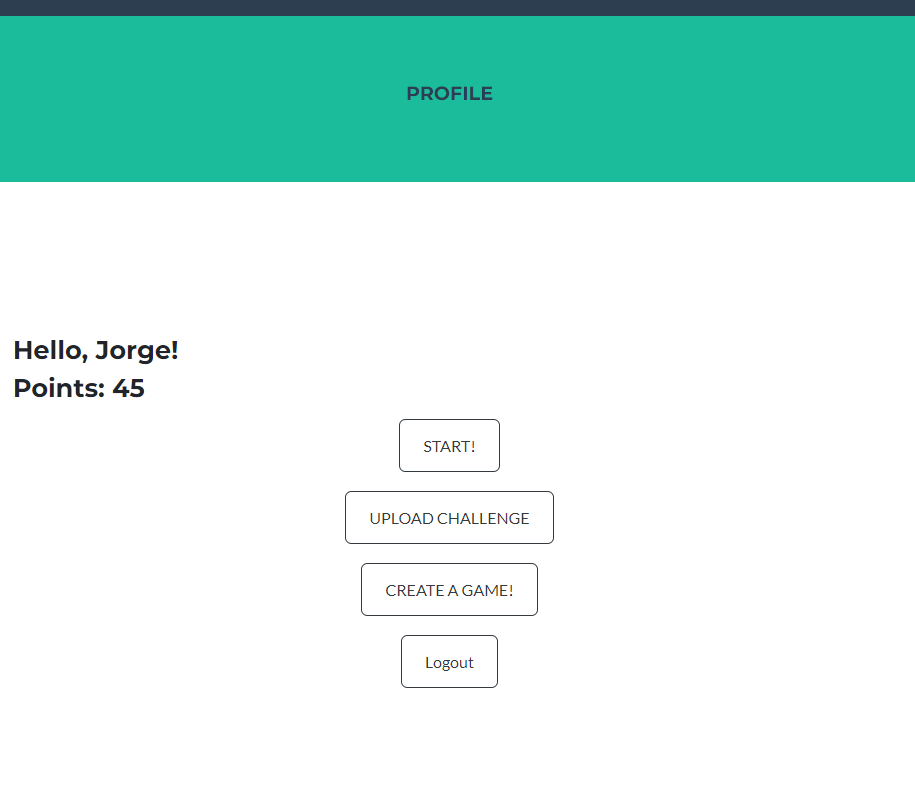
\includegraphics[width=16cm, keepaspectratio]{img/profile_html.png}
	\caption{Perfil del usuario.}\label{fig:profile}
\end{figure}

\section{Subida de retos}
Si el usuario ha accedido hasta la página de subida de retos, para poder continuar, deberá rellenar un formulario. Se supone que esta funcionalidad solo se le concede a usuarios de confianza, por tanto, aunque el formulario sí que sea resistente a intentos de subida con campos vacíos, no está diseñado para comprobar que los campos rellenados sean coherentes con lo que se espera recibir. Se asume que el usuario al que se le han concedido estos permisos subirá retos coherentes y de manera responsable. También hay que tener en cuenta que, en este punto, se pueden subir imágenes que se guardarán directamente en la máquina que hospeda la web en Heroku, por tanto, si esto estuviera abierto al público en general, se podría generar una sobrecarga de memoria en la máquina que hospeda la web.
El formulario es bastante claro con los campos a rellenar, la imagen la debemos seleccionar haciendo click en el campo que pide la misma, y subiendo la imagen deseada desde la memoria del ordenador desde el que se esté haciendo la solicitud. 
Para completar correctamente la subida de reto es necesario pulsar el botón situado al final de la página. 

\begin{figure}
	\centering
	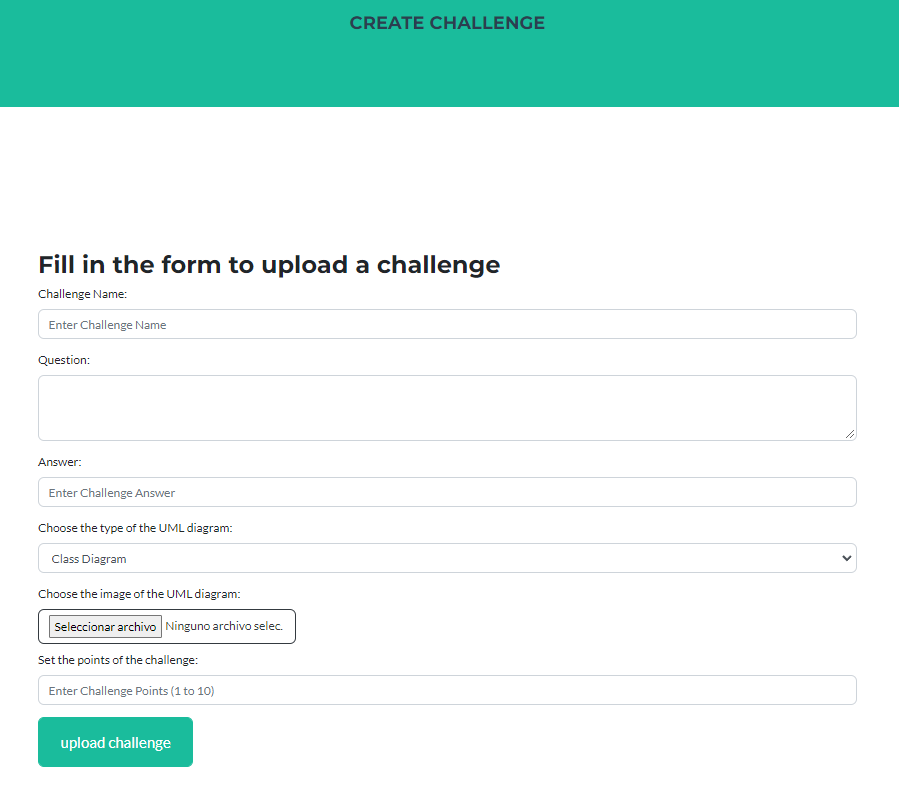
\includegraphics[width=16cm, keepaspectratio]{img/create_challenge_html.png}
	\caption{Formulario de subida de retos.}\label{fig:create_challenge}
\end{figure}

\section{Creación de juegos}
Esta página funciona de manera muy parecida a la anterior, y solo tendrá acceso aquel usurario que se ha registrado a través del inicio de sesión. Consiste, al igual que en el módulo anterior, en rellenar un formulario sencillo. Es necesario añadir un título para el juego y seleccionar en el menú desplegable uno o varios retos que compondrán dicho juego. 
Para completar la subida del juego hay que pulsar el botón que hay al final de la página. 

\begin{figure}
	\centering
	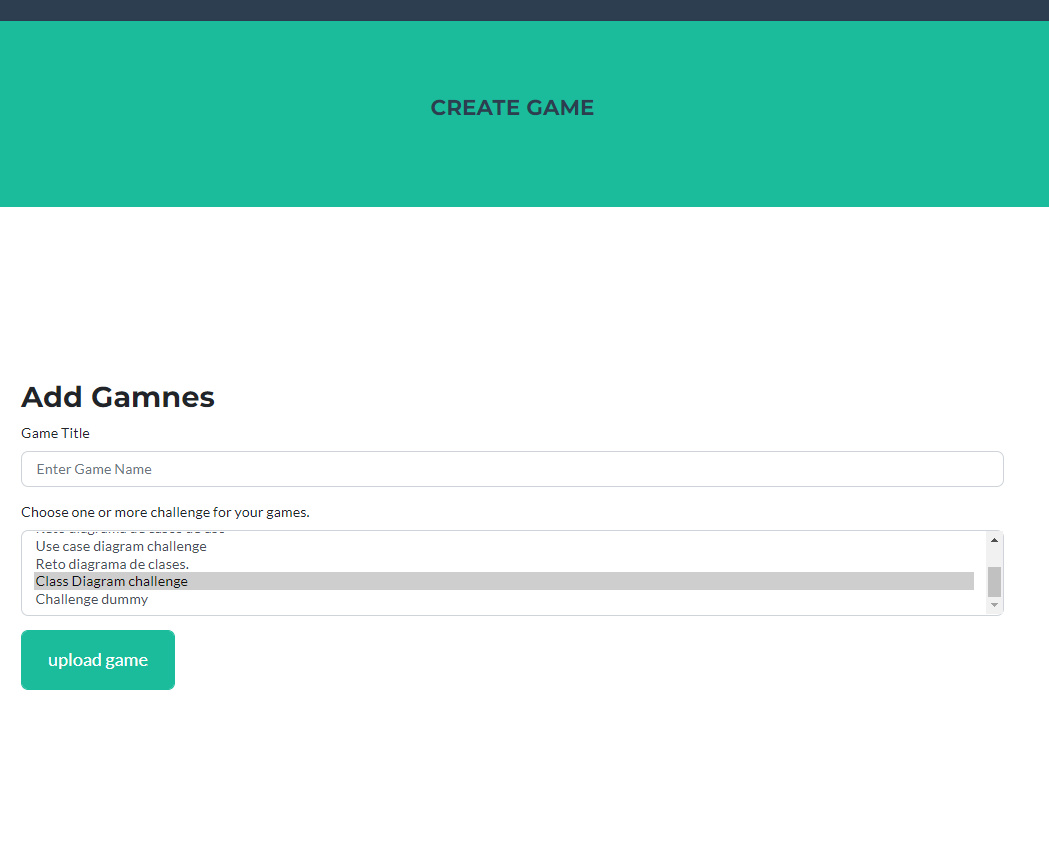
\includegraphics[width=16cm, keepaspectratio]{img/create_game_html.png}
	\caption{Formulario de creación de juegos.}\label{fig:create_game}
\end{figure}



%%%%%%%%%%%%%%%%%%%%%%%%%%%%%%%%%%%%%%%%%%%%%%%%%%%%%%%%%%%%%%%%%%%%%%%%%%%%%%%%
%%%%%%%%%%%%%%%%%%%%%%%%%%%%%%%%%%%%%%%%%%%%%%%%%%%%%%%%%%%%%%%%%%%%%%%%%%%%%%%%
% EXPERIMENTOS Y VALIDACIÓN %
%%%%%%%%%%%%%%%%%%%%%%%%%%%%%%%%%%%%%%%%%%%%%%%%%%%%%%%%%%%%%%%%%%%%%%%%%%%%%%%%

\cleardoublepage


\chapter{Experimentos y validación}

\label{chap:validacion}
%Describe los experimentos y casos de test que tuviste que implementar para validar tus resultados. 
%Incluye también los resultados de validación que permiten afirmar que tus resultados son correctos. 

El fin de este proyecto es ofrecer una aplicación web que pueda ser utilizada por docentes y estudiantes para realizar dos tareas específicas: Poder crear juegos compuestos por gymkhanas y poder resolver los mismos.

Los primeros experimentos y validaciones se llevaron a cabo en dos fases; la fase de validación en local, sobre WSL, y la fase de validación con el software desplegado en Heroku.


\section{Validación sobre un entorno WSL.}

Para validar de manera prácticamente inmediata el desarrollo de nuevas funcionalidades o los cambios que se han ido añadiendo, se ha utilizado, en este caso, un subsistema de Windows para Linux, del que se habla más en profundidad en la sección \ref{sec:WSL} de este documento. Este tipo de entorno es ideal para el desarrollo de software debido a que puedes emular un entorno con el SO y con las dependencias y librerías similares a las que tendría un servidor Linux donde se acabará alojando el código de la aplicación. 

A nivel de control de versiones, las validaciones sobre WSL se han hecho en la rama \emph{develop}, donde se añadían las modificaciones de software que requería el proyecto en cada punto. 

De esta manera, durante el desarrollo se ha validado el correcto funcionamiento de cada característica, de manera individual y progresiva, en un servidor web desplegado en el \emph{localhost}. Una vez aprobadas las nuevas funcionalidades y cambios se llevaba a cabo la segunda fase de validación. 
	
\section{Validación en la plataforma Heroku.}

Después de la primera fase de desarrollo y validación se despliega el software en la plataforma Heroku, como se vio en la sección \ref{sec:despliegue} de este proyecto. 

Hay que remarcar que, antes del despliegue en Heroku, el proyecto requería ciertas modificaciones a nivel de archivos de configuración o referencias a ficheros y rutas internas. Esto es debido a que el software va a alojarse en otra máquina, por tanto, la arquitectura de ficheros no coincide con lo desplegado en el servidor WSL local. Esto es fácilmente manejable gracias al control de versiones de Git, donde la referencia estos ficheros se dejaba ajustada con los parámetros necesarios de WSL en la rama \emph{develop} y en la rama \emph{main} lo correspondiente a las necesidades de la máquina virtualizada de Heroku. De este modo, cada vez que se completaba una fase de validación en local, y se requería emprender una validación en Heroku, era necesario mergear y añadir los últimos cambios hechos sobre el software a la rama \emph{main} del proyecto. Una vez hecho eso, si se encontraba algún problema durante esta fase de validación relacionado con Heroku, su añadían los \emph{bugfix} sobre esta rama. Se muestra un ejemplo de esto en la figura \ref{fig:git_graph.png}.

\begin{figure}
	\centering
	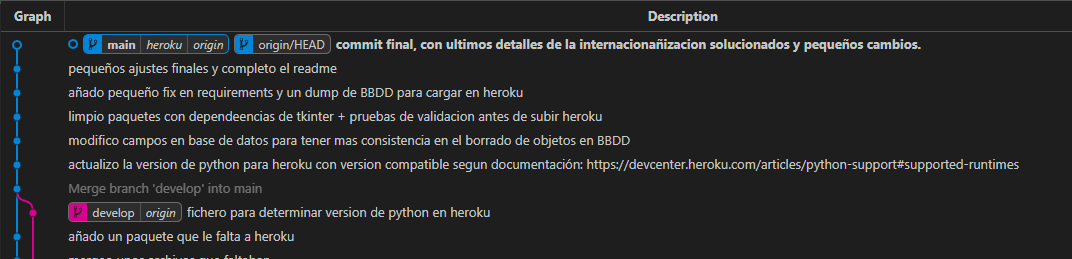
\includegraphics[width=16cm, keepaspectratio]{img/git_graph.png}
	\caption{Gráfico de Git del repositorio.}\label{fig:git_graph.png}
\end{figure}


En ambas fases el proceso de validación era el mismo. A través de pruebas manuales, probando las nuevas funcionalidades y comprobando que no entraban en conflicto con las funcionalidades ya validadas en fases anteriores del desarrollo. Por ejemplo, si se quería validar que funcionaba la creación de juegos o retos, se subía en cada caso un reto ``\emph{dummy}'', cuya única función era comprobar que los flujos de trabajo del software funcionaban correctamente. Esto se ha hecho con todas las funcionalidades requeridas durante el desarrollo del proyecto, hasta alcanzar el resultado actual.


%%%%%%%%%%%%%%%%%%%%%%%%%%%%%%%%%%%%%%%%%%%%%%%%%%%%%%%%%%%%%%%%%%%%%%%%%%%%%%%%
%%%%%%%%%%%%%%%%%%%%%%%%%%%%%%%%%%%%%%%%%%%%%%%%%%%%%%%%%%%%%%%%%%%%%%%%%%%%%%%%
% CONCLUSIONES %
%%%%%%%%%%%%%%%%%%%%%%%%%%%%%%%%%%%%%%%%%%%%%%%%%%%%%%%%%%%%%%%%%%%%%%%%%%%%%%%%

\cleardoublepage


\chapter{Conclusiones}
\label{chap:conclusiones}


\section{Consecución de objetivos}
\label{sec:consecucion-objetivos}

En este proyecto sí se ha conseguido desplegar una aplicación web que puede llenarse de juegos y retos que divulguen sobre el lenguaje de modelado unificado. Se ha hecho desde cero, con tecnologías de código abierto y/o servicios gratuitos. La aplicación es sencilla, limpia y fácil de entender para gente de todas las edades. Se ha conseguido también internacionalizarla usando especificaciones y estándares conocidos por toda la comunidad de desarrolladores.

En cuanto los objetivos específicos: 
\begin{enumerate}
	\item \textbf{Primera versión de la aplicación funcionando en \emph{localhost}.} Este objetivo ha sido alcanzado con creces, ha sido el objetivo más abstracto y con más tareas a realizar. En este objetivo va incluido el diseño inicial del proyecto, elección de los estilos y la mayor parte de lo visto en el Capítulo~\ref{chap:diseño}. Cabe destacar que desde este punto de partida inicial se han añadido diferentes cambios críticos para el proyecto.
	\item \textbf{Agrupación de juegos y retos, y navegación en menú entre ellos.} Para llevar a cabo este objetivo fue necesario reorganizar parte de la estructura de la base de datos inicial, especialmente los campos de \emph{Challenges} y \emph{Games}. También para poder gestionar la navegación entre retos contenidos en juegos se añadieron varias funciones extras en el archivo \emph{utils.py}
	\item \textbf{Internacionalización del proyecto.} Gracias al estándar i18n se ha podido alcanzar este objetivo con relativa facilidad. Fue necesario cambiar prácticamente todos los textos de la plantilla e invertir tiempo en la traducción y compilación de los archivos \emph{.po}, pero considero que es una pieza clave del proyecto y un objetivo alcanzado con éxito.
	\item \textbf{Sistema de gestión de usuarios que puedan subir retos y crear juegos}. Se puede decir que este ha sido el objetivo más complicado del proyecto. Desarrollar un \emph{login} en Django en principio es sencillo, y te da muchas facilidades la documentación, pero en este caso lo complicado era diseñar la aplicación de tal forma que solo ciertos usuarios pudiesen registrarse. El objetivo de estar registrado es poder subir retos, lo que conlleva poder subir archivos a la base de datos del proyecto, y, por tanto, es necesario un control de acceso más restrictivo en este caso. Se decidió en este punto que solo el administrador o administradores del proyecto tengan la potestad de crear usuarios. 
	\item \textbf{Añadir sistema de puntuación}. Para poder cumplir este objetivo fue necesario cambiar la estructura de la base de datos de nuevo y añadir ciertas funciones en \emph{utils.py} para poder gestionar toda la parte de retorno de puntuaciones.  
	\item \textbf{Despliegue de la aplicación y hacerla pública}. Este último objetivo se logró de igual forma que los otros. Llegados a este punto del desarrollo este último fue relativamente sencillo, gracias a la documentación de Heroku y que está diseñado y orientado para ser utilizado en  este tipo de proyectos.  
\end{enumerate}

Gracias a esto, se ha hecho accesible una herramienta que pueden usar docentes y estudiantes de todo el mundo. En contra partida, es esto último lo que no se ha conseguido. En términos generales no se ha logrado que ningún docente o alumno (más allá de pruebas específicas para el proyecto) usen la aplicación desarrollada en este proyecto. No obstante, tanto el código como la aplicación se quedará desplegada en la red de Internet para que se tenga acceso desde cualquier parte del mundo en cualquier momento. 


\section{Aplicación de lo aprendido}
\label{sec:aplicacion}

Este proyecto ha puesto en práctica muchos de los conocimientos enseñados en el Grado en Ingeniería en Sistemas Audiovisuales y Multimedia y también otros adquiridos de manera autodidacta o en el entorno laboral. Especialmente los relacionados con el desarrollo de software.

Se puede decir que las asignaturas que más han aportado en cuanto a conocimientos utilizados en este proyecto es la de Construcción de Servicios y Aplicaciones Audiovisuales en Internet y Protocolos para la Transmisión de Audio y Vídeo en Internet. En estas asignaturas aprendí mucho sobre desarrollo web (HTML, JavaScript y CSS) y programación con Python, aprendiendo a usar la programación orientada a objetos, estructuras de datos, extracción y escritura de información de ficheros y, en general, profesionalizarme con el uso de una herramienta tan potente como es Python. Además, hay que remarcar todo el conocimiento sobre Linux, programación, protocolos de comunicación, arquitectura de sistemas, tratamiento de imágenes y muchos más conocimientos adquiridos en el resto de las asignaturas que han sido indispensables para llevar a cabo este trabajo.

También se han aplicado muchos contenidos de la asignatura optativa Laboratorio de Tecnologías Audiovisuales en la Web que, en mi caso específico yo no cursé, ya que durante la movilidad internacional que realicé, convalidé esa asignatura con otra llamada Databases. No obstante, se me facilitó algunos contenidos docentes de esta asignatura para que me ayudaran en el desarrollo de este proyecto. Al mismo tiempo, la asignatura de base de datos cursada durante la movilidad también me aportó conocimientos que han sido esenciales para entender los modelos de entidad relación y los modelos de bases de datos utilizadas para la aplicación web.

\section{Lecciones aprendidas}
\label{sec:lecciones_aprendidas}
El desarrollo de este trabajo ha servido para reforzar y ampliar conocimientos que adquirí durante la carrera y, además, adquirir otros nuevos y aprender sobre tecnologías y conceptos anteriormente desconocidos para mí. 

\begin{enumerate} 
  \item \textbf{Lenguaje unificado modelado}. El objetivo de este proyecto es tratar de divulgar y expandir conocimientos sobre este lenguaje de modelado y para ello es naturalmente necesario conocer este mismo profundamente. Aunque antes de empezar este proyecto sí que sabía acerca de UML y usado muchos de sus esquemas en varias ocasiones, sabía bastante menos de lo que se hoy en día. La investigación realizada para el desarrollo de este proyecto me ha aportado mucha nueva información, anteriormente desconocida para mí, sobre este lenguaje que considero que me será muy útil en todos los procesos de modelado de software a los que me enfrente en el resto de mi carrera profesional. 
  \item \textbf{Django}. La tecnología principal utilizada en el desarrollo del proyecto ha sido Python y Django. A pesar de que he trabajado anteriormente con Python y es una tecnología en la que me siento cómodo desarrollando, no había desarrollado ningún proyecto Django anterior a este. Creo que esta tecnología es idónea si estás acostumbrado a trabajar con Python y haber podido aprender a usar esta potente herramienta durante el desarrollo de este proyecto me ha a portado mucho para mi \emph{background} profesional con Python. 
  \item \textbf{Diseño de datos}. Enfrentarme al diseño e implementación de una base de datos, teniendo que estudiar bien los campos y las relaciones entre estos para que una aplicación funcione correctamente ha sido un reto nuevo anteriormente desconocido para mí. 
  \item \textbf{Internacionalización y i18n}. Gracias al desarrollo de este proyecto he podido conocer un estándar tan potente y útil como i18n, es una de las tecnologías que más me ha sorprendido descubrir, me parece sencilla, completa y útil en muchos aspectos y considero que es fundamental en prácticamente cualquier proyecto web con ámbito internacional. 
  \item \textbf{Heroku}. También he aprendido bastante sobre Heroku, durante el desarrollo he tenido que leer mucha documentación para llega a entender cómo funciona y poder hacer un despliegue de código limpio. Aprender sobre este tipo de servicios es muy útil ya que fácilmente puedes tener un pequeño proyecto web con acceso mundial y gratuitamente. 
\end{enumerate}


\section{Trabajos futuros}
\label{sec:trabajos_futuros}
Como todos los proyectos web, esta aplicación permite nuevas implementaciones, mejoras y cambios que pueden hacer de \texttt{Gymkhana App} una herramienta más completa, óptima, segura y útil en líneas generales. Algunas de las líneas de trabajo futuras podrían ser las siguientes: 

\begin{itemize}
	\item Hacer más segura la aplicación, de manera que así puedan subir retos y juegos cualquier usuario que se quiera registrar, asegurándose de que con un software automatizado no puedan lanzar cientos de peticiones que puede que haga peligrar la integridad del proyecto.
	\item Hacer compatible la interfaz de usuario con dispositivos móviles y tabletas. Esta aplicación se ha desarrollado para visualizarse en una web a través de navegadores convencionales sobre ordenadores, aunque parte de ella sí es lo que se denomina \emph{responsive}, no se ha enfatizado en hacerla totalmente compatible con dispositivos móviles. 
	\item Ampliar la información que se tiene de un usuario registrado, como por ejemplo los retos ya superados, porcentajes y estadísticas del porcentaje de juegos jugados y por jugar, y otra información que detalle más logros superados y pendientes para jugador. 
	\item Si se logra el primer objetivo de esta lista, se podría implementar el inicio de sesión a través de Google o Facebook con la intención de hacer más sencilla la implicación del usuario con \texttt{Gymkhana App}. 
	\item Evolucionar o mejorar el sistema de retos para que el juego consista en algo más que en dar una respuesta a un reto, algo más interactivo o completo. 
	\item Como todos los proyectos de software, siempre se pueden mejorar la resistencia a errores. Someter la aplicación a una fase de QA\footnote{QA: De las siglas Quality Asurance, consiste en asegurar que el producto final sea de calidad, robusto y funcione correctamente} para asegurar el buen funcionamiento de la aplicación en cualquier caustica a la que esté sometido el programa.
	\item Conseguir difundir el uso de la aplicación entre docentes y alumnos y obtener de estos un buen muestreo tanto de opiniones y resultados para comprobar si realmente \texttt{Gymkhana App} cumple el propósito de familiarizar y ayudar a comprender de mejor manera conceptos del lenguaje de modelado unificado. 
	
\end{itemize}

%Para eso, en Linux tenemos aspell, que se ejecuta de la siguiente manera desde la línea de \emph{shell}:
%\begin{verbatim}
%	aspell --lang=es_ES -c memoria.tex
%\end{verbatim}


%%%%%%%%%%%%%%%%%%%%%%%%%%%%%%%%%%%%%%%%%%%%%%%%%%%%%%%%%%%%%%%%%%%%%%%%%%%%%%%%
%%%%%%%%%%%%%%%%%%%%%%%%%%%%%%%%%%%%%%%%%%%%%%%%%%%%%%%%%%%%%%%%%%%%%%%%%%%%%%%%
% APÉNDICE(S) %
%%%%%%%%%%%%%%%%%%%%%%%%%%%%%%%%%%%%%%%%%%%%%%%%%%%%%%%%%%%%%%%%%%%%%%%%%%%%%%%%

\cleardoublepage
\appendix

\chapter{Anexo I: Ejemplos de Diagramas UML}
\label{app:diagramas}
% Contenido del anexo I

\section{Diagrama de clases}
En este diagrama de clases, hay una clase padre y dos clases hijas. En este caso la clase padre cuenta con unos atributos y métodos comunes, los cuales comparte con las clases hijas. Las clases hijas en cambio tienen cada una unos atributos y métodos que no pueden compartir entre ellas ni con la clase padre.
\begin{figure}
	\centering
	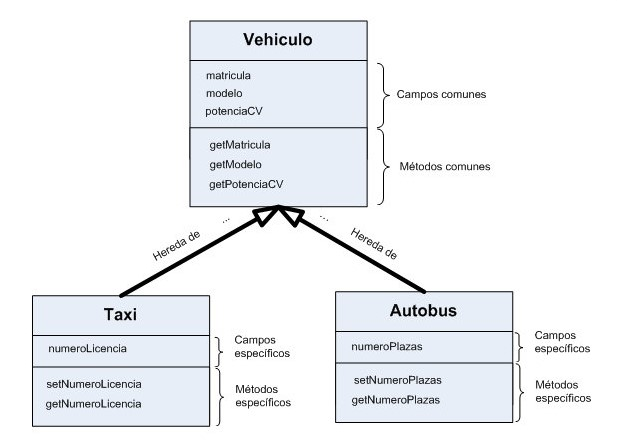
\includegraphics[width=14cm, keepaspectratio]{img/diagrama_clases.png}
	\caption{Ejemplo de diagrama de clases.}\label{fig:diagrama_clases}
\end{figure}

\section{Diagrama de objetos}
Los diagramas de objetos están fuertemente relacionados con los diagramas de clases, tanto es así que hasta comparten símbolos y figuras. Básicamente para seguir con el objeto anterior de los vehículos, en este ejemplo se puede ver los datos o ``fotografía'' de un objeto del sistema en un momento determinado del tiempo. 
\begin{figure}
	\centering
	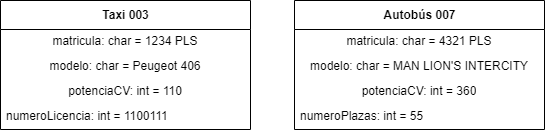
\includegraphics[width=14cm, keepaspectratio]{img/diagrama_objetos.png}
	\caption{Ejemplo de diagrama de objetos.}\label{fig:diagrama_objetos}
\end{figure}

\section{Diagrama de despliegue}
Este diagrama de despliegue modela la arquitectura en tiempo de ejecución de un sistema. Se muestra la configuración de los elementos de hardware, identificados como nodos. Y muestra las trazas de elementos y artefactos del software en estos nodos. 
\begin{figure}
	\centering
	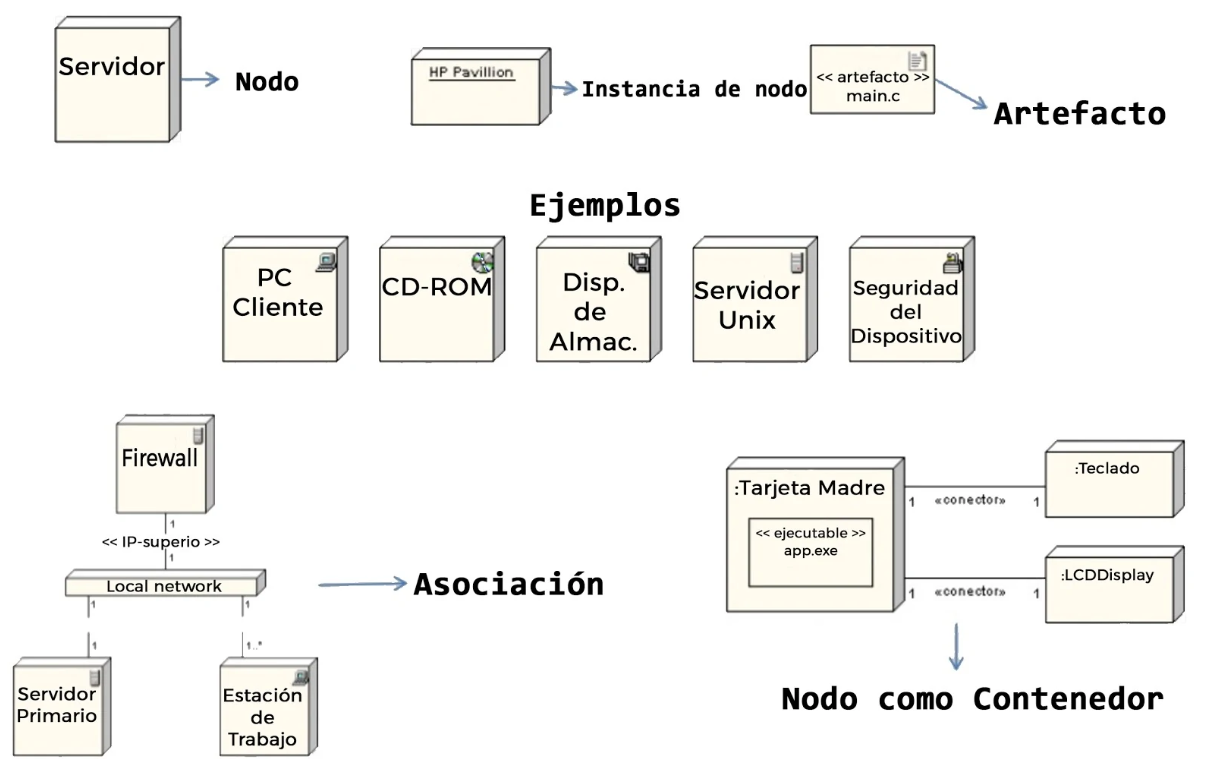
\includegraphics[width=16cm, keepaspectratio]{img/diagrama_despliegue.png}
	\caption{Ejemplo de diagrama de despliegue.}\label{fig:diagrama_despliegue}
\end{figure}

\section{Diagrama de componentes}
En este diagrama de componentes se puede visualizar la estructura y la funcionalidad de un software de correo electrónico. Muestra la interacción a través de sus tres interfaces. La línea discontinua etiquetada con ``use'' indica que el usuario es dependiente de esa interfaz (management port) para supervisar y administrar el correcto funcionamiento del sistema.
\begin{figure}
	\centering
	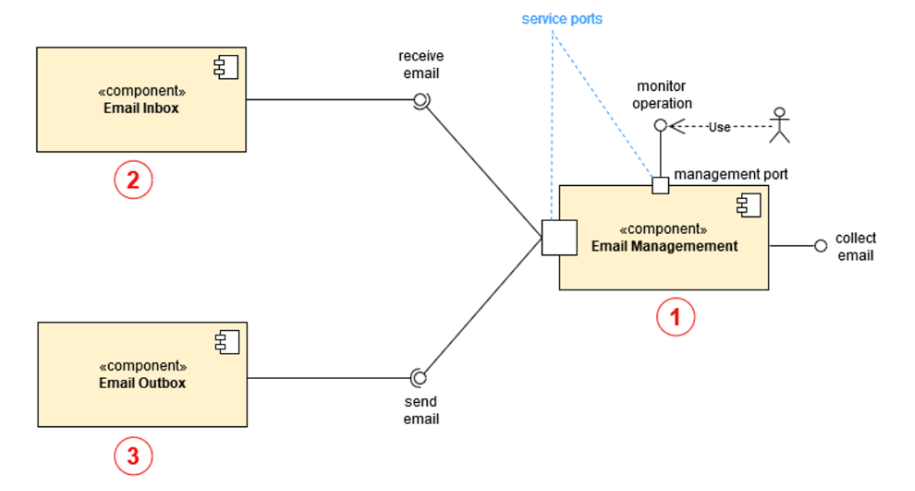
\includegraphics[width=18cm, keepaspectratio]{img/diagrama_componentes.png}
	\caption{Ejemplo diagrama de componentes.}\label{fig:diagrama_componentes}
\end{figure}

\section{Diagrama de paquetes}
En este ejemplo de diagrama de paquetes tiene la intención de mostrar la organización y disposición de los diferentes elementos que componen una aplicación web para compras. Las carpetas representan la anidación de elementos del software, y estas a la vez se organizan jerárquicamente dentro del diagrama. 
\begin{figure}
	\centering
	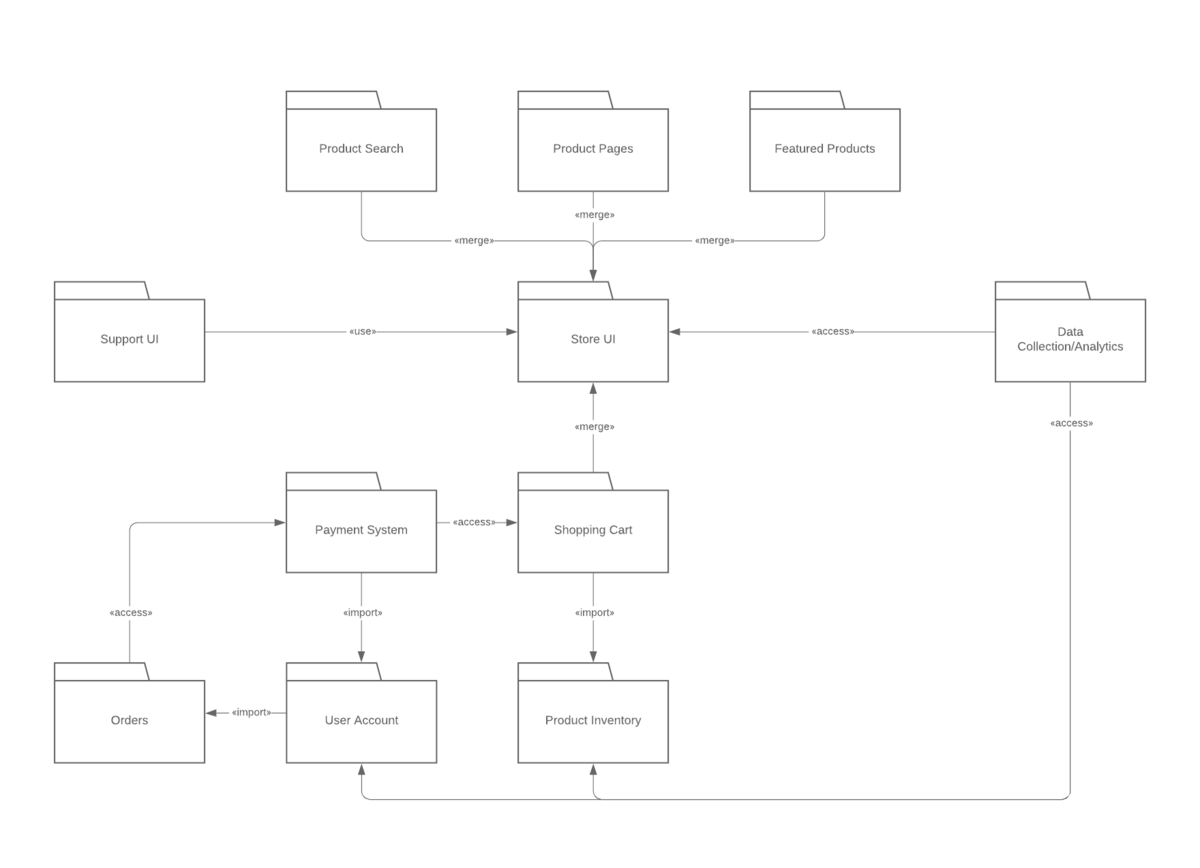
\includegraphics[width=14cm, keepaspectratio]{img/diagrama_paquetes.png}
	\caption{Ejemplo diagrama de paquetes.}\label{fig:diagrama_paquetes}
\end{figure}

\section{Diagrama de estructura compuesta}
En este ejemplo podemos apreciar el diagrama de estructura compuesta de un sistema contraincendios. Se puede ver que la unidad central de control está compuesta por componentes más pequeños (sirena, aspersores, sensores, monitores...), que a su vez pertenecen al sistema general.
\begin{figure}
	\centering
	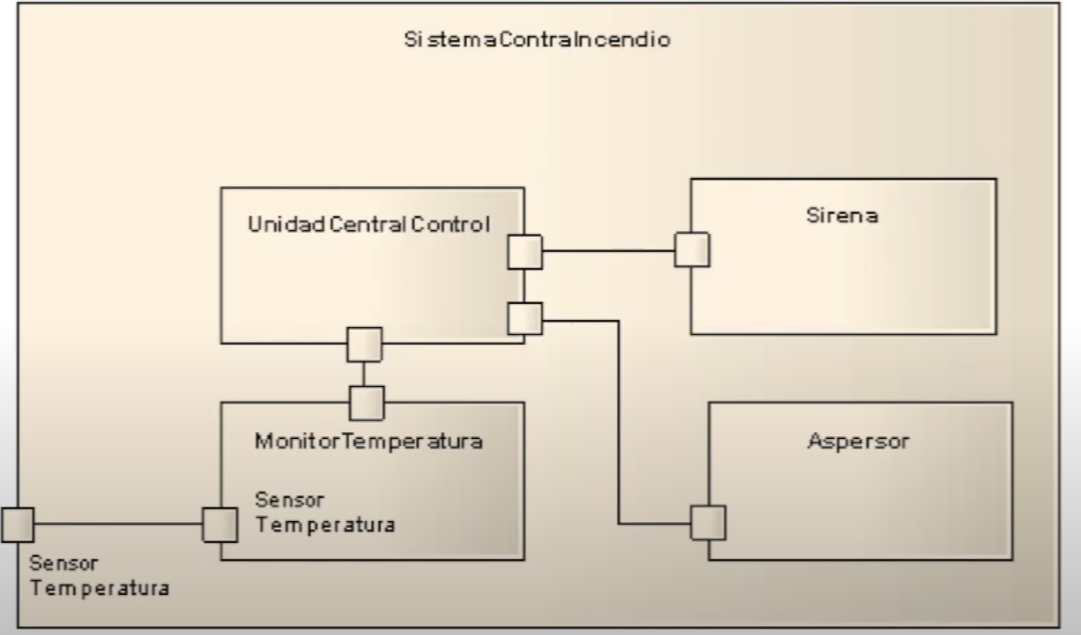
\includegraphics[width=12cm, keepaspectratio]{img/diagrama_estructura_compuesta.png}
	\caption{Ejemplo diagrama de estructura compuesta.}\label{fig:diagrama_estructura_compuesta}
\end{figure}

\section{Diagrama de actividad}
Este ejemplo de diagrama es uno de los usados para los retos de Gymkhana App. Este tipo de diagramas es de los más conocidos, en este caso se trata de seguir el flujo de trabajo, pudiendo actuar de distinta manera dependiendo de las respuestas del sistema a diferentes preguntas (representadas con rombos). 
\begin{figure}
	\centering
	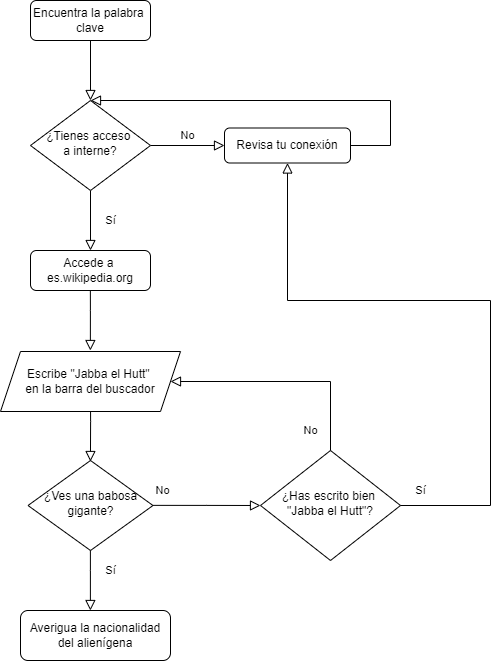
\includegraphics[width=10cm, keepaspectratio]{img/diagrama_actividad.png}
	\caption{Ejemplo diagrama de actividad.}\label{fig:diiagrama_actividad}
\end{figure}

\section{Diagrama de casos de uso}
Este ejemplo modela la funcionalidad de un ``Sistema Apocalipsis Zombie'' con los diferentes casos de uso representado con elipses. Se muestra también la interacción que tiene el actor (superviviente) con el sistema. Este diagrama ha sido diseñado para uno de los primeros retos de la aplicación Gymkhana App.
\begin{figure}
	\centering
	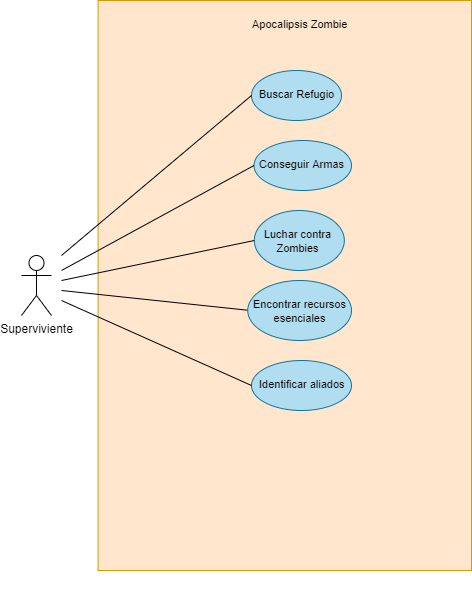
\includegraphics[height=18cm,width=12cm, keepaspectratio]{img/diagrama_casos_uso.png}
	\caption{Ejemplo diagrama casos de uso.}\label{fig:diagrama_casos_uso}
\end{figure}

\section{Diagrama de máquina de estados}
En este ejemplo se muestra un diagrama del proceso de inscripción y finalización de una asignatura de la universidad. Se puede ver como el estado pasa de tratar de apuntarse a una asignatura, a poder matricularte en esta y pasar los exámenes finales. 
\begin{figure}
	\centering
	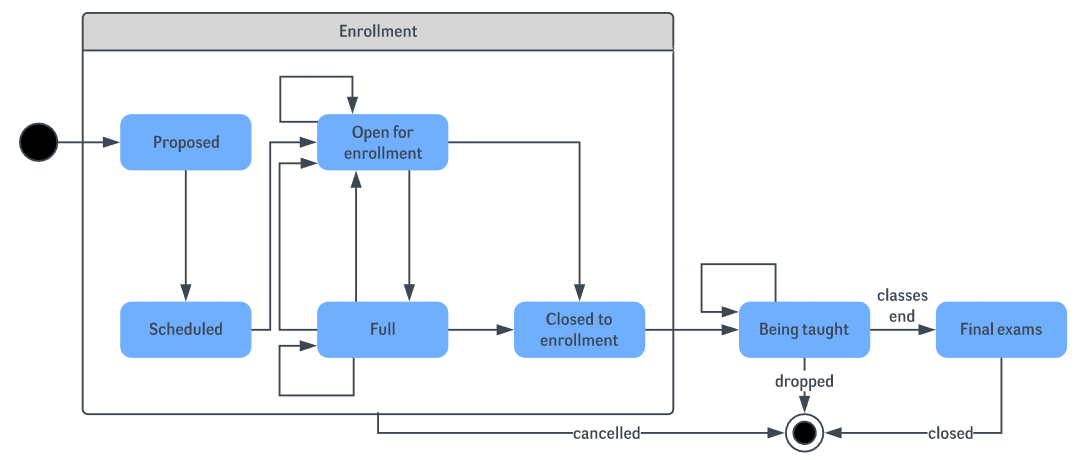
\includegraphics[width=16cm, keepaspectratio]{img/diagrama_maquina_estados.png}
	\caption{Ejemplo diagrama de máquina de estados.}\label{fig:diagrama_maquina_estados}
\end{figure}

\section{Diagrama de interacción}
Como dentro de estos tipos de diagramas se pueden clasificar cuatro más, en este apartado se aportan ejemplos sencillos de alguno de ellos.

Los diagramas de colaboración se centran en los aspectos estructurales y la arquitectura de los objetos de un software. En el ejemplo se muestra el flujo de organización de una tienda online, con el tipo de mensajes y de llamadas que se hacen entre los objetos del sistema. 
\begin{figure}
	\centering
	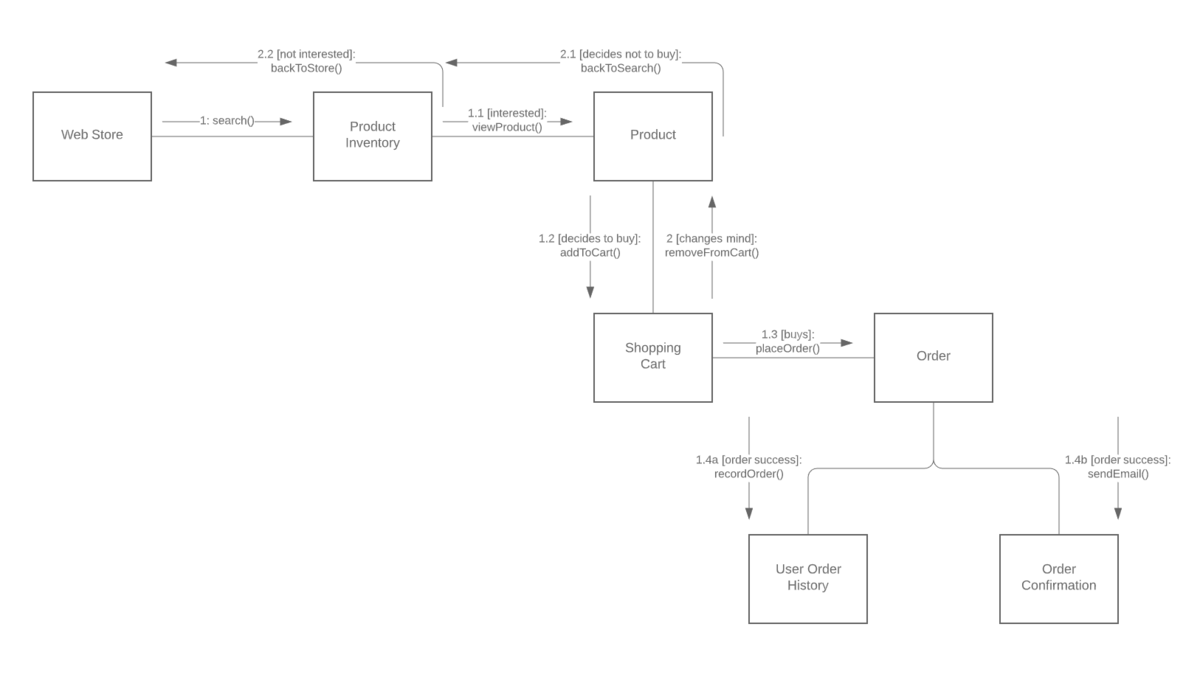
\includegraphics[width=14cm, keepaspectratio]{img/diagrama_colaboracion.png}
	\caption{Ejemplo diagrama de colaboración}\label{fig:diagrama_colaboracion}
\end{figure}

Los diagramas de secuencia se centrar en representa las interacciones entre los eventos de un sistema. En el ejemplo se muestra la secuencia de eventos de un software de manejo de una agenda, enlazada a una dirección de correo electrónico.
\begin{figure}
	\centering
	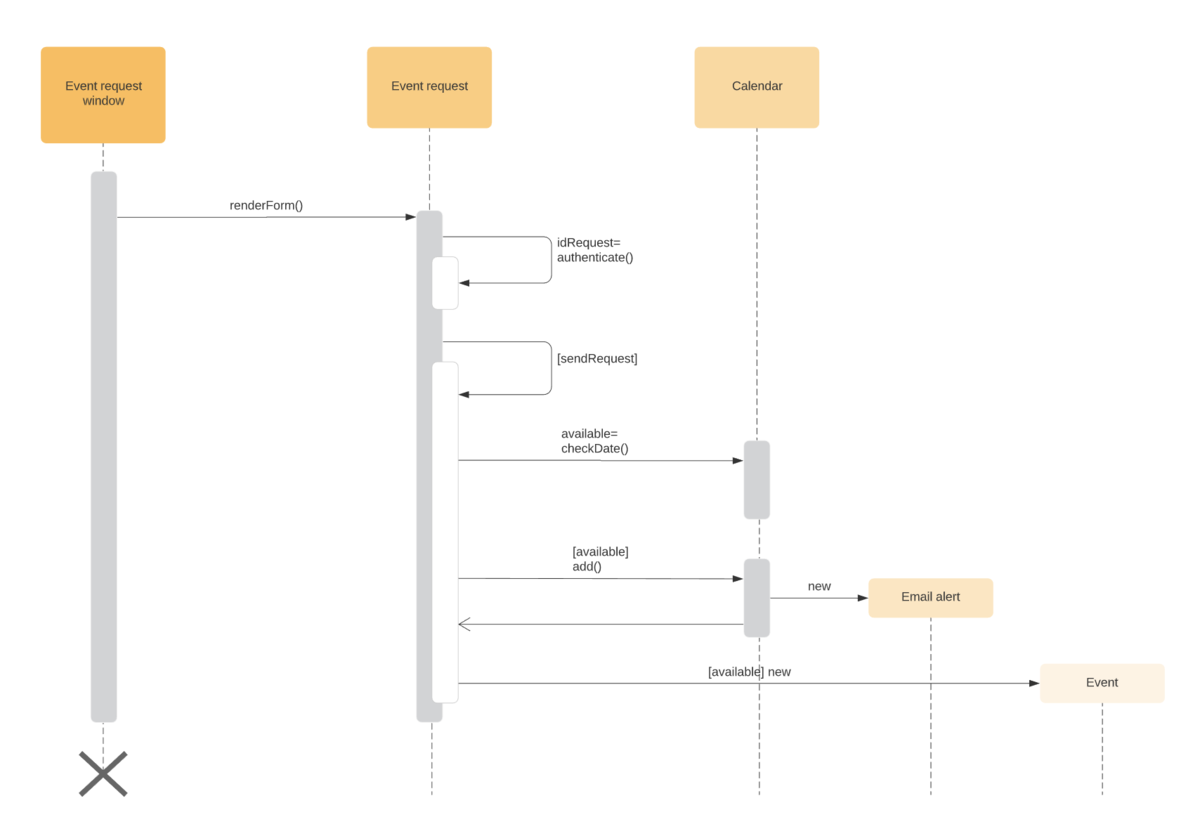
\includegraphics[width=14cm, keepaspectratio]{img/diagrama_secuencia.png}
	\caption{Ejemplo diagrama de secuencia}\label{fig:diagrama_secuencia}
\end{figure}

Los diagramas de tiempos se unas para representar la línea de vida de un objeto en una instancia y en el tiempo. Se representa los cambios con nivel alto y bajo con señales. En el ejemplo se puede ver un diagrama del comportamiento de los objetos que forman un sistema contraincendios.
\begin{figure}
	\centering
	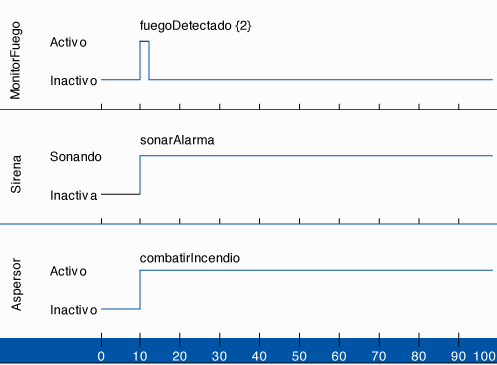
\includegraphics[width=12cm, keepaspectratio]{img/diagrama_tiempos.png}
	\caption{Ejemplo diagrama de tiempos.}\label{fig:diagrama_tiempos}
\end{figure}


%%%%%%%%%%%%%%%%%%%%%%%%%%%%%%%%%%%%%%%%%%%%%%%%%%%%%%%%%%%%%%%%%%%%%%%%%%%%%%%%
%%%%%%%%%%%%%%%%%%%%%%%%%%%%%%%%%%%%%%%%%%%%%%%%%%%%%%%%%%%%%%%%%%%%%%%%%%%%%%%%
% BIBLIOGRAFIA %
%%%%%%%%%%%%%%%%%%%%%%%%%%%%%%%%%%%%%%%%%%%%%%%%%%%%%%%%%%%%%%%%%%%%%%%%%%%%%%%%

\cleardoublepage

\bibliographystyle{abbrv}
\bibliography{memoria}  % memoria.bib es el nombre del fichero que contiene
% las referencias bibliográficas.

\end{document}
